\documentclass[UKenglish]{ifimaster}

\usepackage{thesisstyle}

\addbibresource{references.bib}
\addbibresource{proceedings.bib}

\title{Automated Assessment of Norwegian L2 Essays}
\subtitle{Using Multi-task Learning}
\author{Stig Johan Berggren}

% \renewcommand*\rmdefault{ptm}

\begin{document}

\duoforside[
  dept={Department of Informatics},
  program={Language and Communication},
  long
]

\frontmatter{}

\tableofcontents{}
\listoffigures{}
\listoftables{}

% \chapter*{Preface}

\mainmatter{}

\section{Background}

In this essay, I cover some of the background concerning the Native Language
Identification and Automated assessment tasks, which are well studied in the
field of natural language processing (NLP). I will examine how these tasks
may be addressed simultaneously using multi-task learning and some approaches
to the separate tasks that have been found useful in previous work. The topic
of multi-task learning will also be discussed in the essay.

The first section covers background related to machine learning and different
neural methods. Then, we will look at the properties of learner language, and
the specific tasks of automated scoring and native language identification.
We will also look at a selection of datasets of learner language that have
been used for these tasks previously.


\section{Tasks and machine learning}

Machine learning (ML) is a field that covers a wide range of different
techniques and algorithms for ``teaching'' computers to perform well at a
range of tasks. Examples of tasks may be categorizing a document or detecting
an object in an image. Techniques in machine learning are often categorized
under labels such as \emph{supervised learning}, \emph{unsupervised
learning}, and \emph{reinforcement learning}.

The first two are applicable when we have training data available. Supervised
learning utilizes a set of training examples with target labels in order to
train a model that predict true labels for new, unseen data. In the essay
scoring task discussed below, for instance, training data consists of essays
that already have assigned a grade, and the resulting, trained model should
be able to assign a ``correct'' grade to any essay, including those it has
never seen during training.

Unsupervised learning is a range of techniques which do not use target labels
in training, but are still able to ``learn'' useful representations and
groupings of the training data. Unsupervised learning can be part of a more
complex model, for instance when using embeddings as feature representations
in a neural network. Embeddings map sparse features (e.g. words/tokens) to a
dense, low-dimensional space, using contexts to discover what tokens are
similar and should exist close to each other in this \emph{embedding space}.

Many machine learning algorithms are based on statistical modelling and
concepts from linear algebra, with low-level routines such as matrix
multiplication being central to the algorithms.

In the field of natural language processing, algorithms in the neural network
family are gaining ground on the more ``traditional models'' in the field,
which have generally been linear models such as support vector machines and
logistic regression \autocite[345]{goldberg2016primer}. Compared to the
traditional models, neural networks often require less focus on feature
design and hand-crafting features. On the other hand, feature representations
such as word embeddings are important.


\subsection{Neural networks}

Neural networks is a family of machine learning models. These models are
based upon units often referred to as ``neurons'', which are capable of
computing a weighted sum of inputs and applying a non-linear \emph{activation
function} to the result. The networks are usually trained with supervised
learning, where the performance on training samples is measured using an
\emph{objective} function or \emph{loss} function, which is minimized by
backpropagation. In order for backpropagation to work, it is crucial that the
activation function is differentiable.

One of the simplest models in the neural networks family is the perceptron.
It is only capable of calculating a weighted sum across a feature vector and
applying a threshold function. This threshold function is not differentiable,
and the perceptron is therefore not trained with backpropagation.
Historically, one of the most used activation functions is the sigmoid
function: \(s(x) = {(1 + e^{-x})^{-1}}\). Nowadays, one of the most common
activations is the rectified linear unit (ReLU): \(f(x) = \max(x, 0)\). ReLU
is, strictly speaking, not differentiable, because of its hinge at $x = 0$.
Regardless it works well in practice, since almost all pre-activation values
will be different from zero. The zero case can be treated as a special case,
to avoid undefined values.

\subsubsection{Multi-layer perceptron}

\begin{figure}
  \centering
  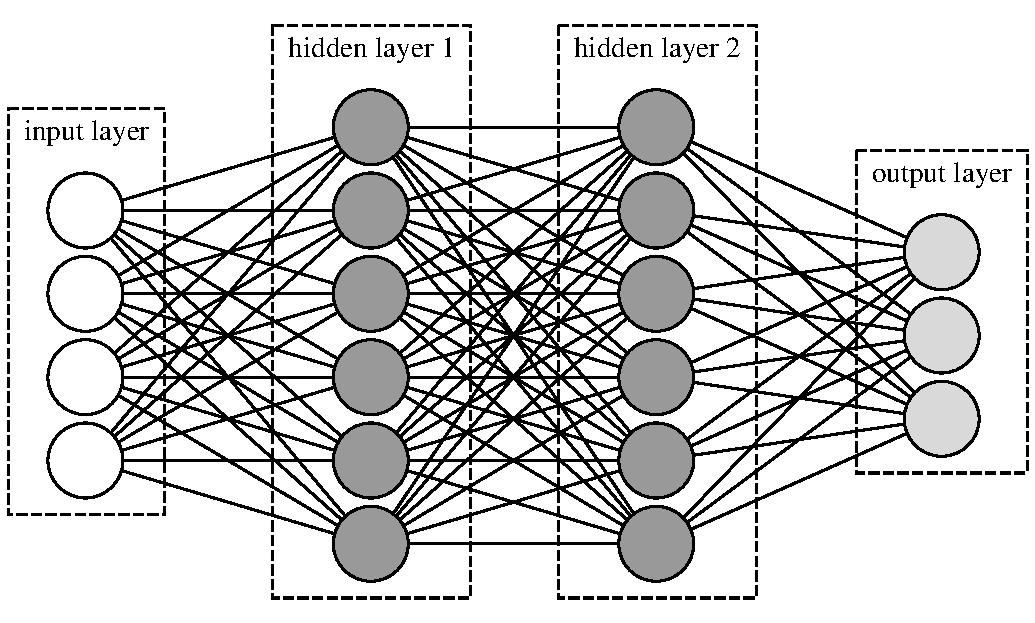
\includegraphics[width=0.8\textwidth]{graph}
  \caption{A fully connected feed-forward neural network with four input
  nodes, two hidden layers, and three output nodes.}
  \label{mlp-diagram}
\end{figure}

The ``vanilla'' neural network is the feed-forward network, also known as the
\emph{multi-layer perceptron} (MLP). This model incorporates one or more
hidden layer in-between the input layer (the feature vector) and the output
layer. A diagram of an example MLP with two hidden layers can be seen in
figure \ref{mlp-diagram}. For multi-class prediction, the output layer
typically uses a \emph{softmax} activation. This has the property of
restricting each output value to be in the interval $(0,1)$, and additionally
makes sure all output values sum to $1$. These properties allow the outputted
values to be interpreted as a probability distribution.


\subsubsection{Convolutional neural networks}

Convolutional neural networks (CNN) can exploit local patterns in the input,
unlike the MLP, which has no way to identify elements of the input layer as
being ``close'' to each other in any sort of measure. CNNs use convolutional
layers to make these local relationships explicit.

CNNs are widely employed in image processing models, using
two-di\-men\-sional convolutional layers. These models can often get very
deep, using a number of convolutional layers at different levels in the
network, interspersed with pooling or downsampling layers.

There are also NLP applications where CNNs can be employed. Unlike images,
data in NLP is usually sequential or one-dimensional, but it may be converted
into two dimensions, for example by replacing each word by an embedding
vector.


\subsubsection{Recurrent neural networks}

Recurrent networks (RNN) are suited to sequential data. They make have an
internal \emph{state} that is passed between time steps. A benefit of RNNs is
that they can accept input of any length and also produce sequential output
of any length. This in contrast to feed-forward neural networks, which take a
fixed-length vector as their input.

A long standing problem in training RNNs was that when applying
backpropagation through time, the gradient values can tend toward zero or
diverge because of multiplication across many time steps. This is known as
the \emph{vanishing} and \emph{exploding gradients problem}, respectively.
Mitigation techniques include replacing the units of the network with what's
known as \emph{gated units}, that are especially designed to address these
problems. Gated recurrent units (GRU) and Long short-term memory (LSTM) are
widely used gated units in RNNs.


\subsubsection{Natural language features}

For applications of machine learning in NLP, we often want to use the words
in a document as features. However, the vast number of different words in a
language can lead to inefficient use of memory and computing power if the
words are represented naively, for instance with a one-hot vector encoding
with the vector having the number of dimensions equal to the size of the
lexicon. It is therefore useful to map words to a lower-dimensional
representation, known as an \emph{embedding}.

\sloppy Training embeddings rely on the distributional hypothesis, namely
that words with similar meanings are likely to appear in similar contexts.
Therefore, without prior knowledge of any words in a language, the resulting
embeddings are likely to put words with similar meanings close to each other
in the embedding space. It has also been observed that semantic relations
between words, for instance regarding gender or inflection, corresponds to
defined directions in the embedding space\autocite{mikolov2013linguistic}.
These relations can be found by subtracting word vectors. A famous example of
an emergent analogy learned by the embeddings is: ``Man is to king as woman
is to ...''. In terms of arithmetic on embedding vectors, the embeddings
modelled the analogy as $\vec{king}-\vec{man}+\vec{woman}\approx\vec{queen}$.
\fussy

There exists a number of embedding models, including Word2Vec
\autocite{mikolov2013word2vec} and GloVe \autocite{pennington2014glove}.
These models can be used to compute embeddings based on new training data, or
one may use pre-trained embeddings.

Different approaches to embeddings may be necessary for different languages.
A word-based approach can work well for a relatively analytic language such
as English, but be less suited for agglutinative or synthetic languages,
because of the differing amount of semantic information present in a single
token. A converse problem occurs where a sequence of words is best analyzed
as a single unit.

Another issue is ambiguity, as the process of training embeddings only
considers the form of a word. Homographs like \emph{well}, which can be both
an adverb adn a noun, are each mapped to a single embedding vector, with no
way to distinguish the different meanings of the word.

It is also possible to embed $n$-grams of characters instead of words. A
disadvantage of this approach is that it becomes more difficult to
distinguish words with similar spelling, but different meaning, and it does
not solve the problem of homographs. However, it seems that the embeddings
may still be more robust when encountering spelling mistakes. The embeddings
based on word forms will see ``beautiful'' and ``beutiful'' as completely
separate words, while there still exists similarities between them on the
level of characters: they share a good portion of their $n$-grams. Another
advantage might be the possibility of accessing semantic meaning at a
sub-word level, including prefixes and suffixes.

For representing a document non-sequentially, a common approach is to use
continuous bag-of-words (CBOW). This is the sum or average of embedding
vectors for all active features \autocite[352]{goldberg2016primer}. CBOW thus
disregards some information, including order and whether features occur close
to each other in the document.


\subsection{Multi-task learning}

Multi-task learning refers to optimizing a target function for two or more
different tasks simultaneously \autocite{ruder17overview}. One benefit of
this approach is increased generalization. Intuitively, this is feasible
because the neural network needs to find a representation which is useful for
all the tasks it is optimizing on, and thus is less likely to pick up noise
in the data than it might be when only considering a single task. A
representation that is useful to different tasks is more likely to be able to
generalize, not only to data beyond the training data, but to new tasks which
were not part of the training process as well.

In practice, for neural networks, the tasks in question share some of the
inner layers of the network, but have separate output layers. This is called
parameter sharing. Another approach is to keep different parameters for each
of the tasks, but add a regularization loss that prevents the parameters from
diverging too much from each other. The output layers are not necessarily at
the same depth. A low-level auxiliary task can have its output layer rather
early while the main task uses more hidden layers. In the backwards pass,
losses at all the output layers should be minimized.

\textcite{ruder17} lists several tasks in natural language processing that
have been subject of experiments with multi-task learning, including machine
translation, speech recognition, semantic parsing and chunking. These tasks
have been jointly trained with auxiliary tasks such as predicting the next
word, recognizing phonemes, part-of-speech tagging, and more. Among others,
the author cites \textcite{pappas17}, who used multi-task learning to train a
document classifier using 8 different languages, sharing parameters between
the models for different languages. The model they used for this was a
hierarchical attention network.

\textcite{alonso17} investigated the effect of different auxiliary tasks and
combinations of these on a LSTM (Long Short-Term Memory) recurrent network
for sequence labelling tasks. The main tasks they considered in the study
were labelling semantic frames, semantic supersenses, named entity
recognition, ontological types for senses and Multi-Perspective Question
Answering.

They used an auxiliary task called \textsc{FreqBin}, whose objective is to
predict the log frequency of a word, discretized into a number of bins. This
study tried a new binning strategy which improved the utility of
\textsc{FreqBin} as an auxiliary task compared with previously examined
strategies. While the previous variants took the logarithm of the token's
frequency in a chosen base and rounded down to the nearest integer, the new
strategy ranked all tokens by frequency grouped them into labels by a given
quantile. In the study, they used $k=5$, yielding 5 \textsc{FreqBin} labels
with the same number of examples each.


\section{Learner language}

In the linguistic field of second language acquisition (SLA), linguists have
described characteristics of the language of people who are learning a second
language. It is common to refer to a person's first language(s), that is the
language(s) they learned when they first started to speak, as L1, and any
languages acquired later in life as L2. Since language acquisition is a
gradual process, we can speak of an \emph{interlanguage}, which is an
idiolect with systematic rules belonging to the learner in question, but
which is different from their target language. Interlanguage is not stable,
but changes as part of a learner's acquisition process
\autocite[358]{myers-scotton}.

Interlanguage can show influences from the learner's L1 in several respects,
for instance intonation and produced phonemes in pronunciation, syntactic
mistakes like inflection and word order, or even the literal translation of
idioms that do not exist in the same form in the target language. The study
of linguistic \emph{transfer} is an attempt to understand these influences.


\subsection{Automated assessment}

Assessment of proficiency, or automatic essay scoring (AES), has been framed
as a supervised learning task, using a corpus of learner texts that have each
been labelled with a proficiency rating. Automating the assessment task can
benefit applications in language education. People learning a new second
language will benefit from feedback as to which proficiency level they might
be on, for instance in relation to the Common European Framework of Reference
for Languages (the European Framework or CEFR). This may help people who want
to take language examination to find the appropriate timing and level of
testing, since an examination can be both an economical and logistical
inconvenience. Automation also allows students to receive feedback quicker
and more frequently.

Previous work by \textcite{vajjala17} uses the TOEFL11 corpus of non-native
English \autocite{blanchard13} and the First Certificate of English (FCE)
corpus \autocite{yannakoudakis2011new}. This study examines which features
may be most informative in relation to the task, and whether these are the
same features for different datasets. \citeauthor{vajjala17} uses a number of
linguistic features for the task, including several different measures for
the lexical diversity, distribution of part-of-speech (POS) tags, and
syntactic complexity. The models in the study utilize up to 116 different
features. Applied pre-processing includes syntactic parsing of sentences in
order to extract features from the parse trees. These syntactic features
include measures of average sentence length, clauses per sentence, the height
of the parse tree etc. Several of these features were based on previous work
on measuring syntactic complexity in L2 writing by
\textcite{lu2010automatic}.

Other features are designed to capture discourse properties of the text,
based on reference chains. The English language has different ways of
referring to previous information in a discourse, which is a core element of
fluent language use. For instance, the definite/indefinite distinction is a
way to reference previous information in English. This is not the case
cross-linguistically, so features like this are language-specific.
\citeauthor{vajjala17}'s features are measures of the proportions of
different pronoun types, determiners and definite noun phrases, and more, in
a reference chain, along with the average length of a reference chain.

Notably, the author did not use word or POS $n$-grams as features in the
study. The reasons given for this is that the sparse nature of $n$-gram
features make them hard to interpret, and they can introduce topic bias to
the model. The essays are written on different topics, making it likely that
certain words indicate the topic of an essay. $n$-grams can model errors
relative to the learner's target language, but she already uses features
designed to model this. Nor are character $n$-grams used as features here,
though they are generally widely used in a various NLP applications.
\citeauthor{vajjala17} also experimented with using the writing prompt and
the native language (L1) of the text's author as features.

The author trained a number of different models using different subsets of
the features. All models are linear classifiers trained with the Sequential
Minimal Optimization algorithm, a variant of support vector machines. The
model that achieved highest accuracy in the study was one that incorporated
all the features, yielding an accuracy of 73.2~\% on TOEFL11. Removing the
prompt and L1 as features resulted in a tiny drop in accuracy down to
73.0~\%.

The length of the text turned out to be one of the most informative features
in both the datasets used. However, text length correlated positively with
proficiency on TOEFL11, but negatively on the FCE corpus.


\subsection{Native Language Identification}

Native Language Identification (NLI) is the task of predicting the native
language of an author based on a text written in one of the author's second
languages (L2). The task is dependent on systematic differences between
interlanguages for learners with the same target language, but different L1s.
The feasibility of this task proves intrinsically that these systematic
differences exist, as linguists studying transfer try to explain.


\subsubsection{Shared tasks in NLI}

NLI has been the subject of three shared tasks, in 2013
\autocite{tetreault2013report}, 2016 \autocite{schuller2016interspeech} and
2017 \autocite{nli17}. The 2013 shared task used only written documents,
whereas the 2016 shared task was audio data only. Lastly, the latest shared
task in 2017 contained both written and spoken documents. Teams participating
in 2017 could choose between three tracks corresponding to written data only,
spoken data only, or both. Only teams participating in the first track, using
written data only, are considered below.

The written documents in the task was English L2 essays, written by learners
with 11 different L1s. The best-performing system in the track using only
written essays had a macro-averaged F1 score of 0.8818, using stacked
classifiers combining logistic regression on sentences with a support vector
machine (SVM) meta-classifier \autocite{cimino17}.

The best performing team which used neural networks was \textcite{li17}, who
used a multi-layer perceptron meta-classifier to combine outputs from SVM
base classifiers, and reported a F1 score of 0.8654. Another team
experimented with different neural network architectures, including RNNs and
a CNN variant known as a deep residual network \autocite{bjerva2017neural}.
Their best result was with a stacked model, combining their different models
with an SVM meta-classifier. Their best ensemble model achieved a F1 score of
0.8323, and used no external resources, i.e. no pre-trained embeddings.


\subsubsection{NLI for Norwegian}

While the shared tasks have been English learner language only, there exists
studies using different corpora with other target languages, among them
Norwegian. Norwegian NLI has been attempted by \textcite{malmasi15}, using
the ASK corpus \autocite{tenfjord06}. In their methodology, they create
artificial documents to train on by segmenting the learner texts into
sentences, then putting all the sentences from learners with the same L1 into
a bag and sampling sentences from the bag to create the new documents. Their
rationale for the methodology is that all the resulting documents are of
similar length, and that they eliminate the variation between individual
writers that otherwise might present a stronger signal than the writer's L1
alone.

In a later study \autocite{malmasi17}, they perform an NLI experiment on
several corpora, namely TOEFL11, the Norwegian ASK corpus and the Jinan
Chinese Learner corpus. However, they were not able to utilize the same
features for all the different corpora. For Norwegian, they only use the
features \emph{function word unigrams}, \emph{function word bigrams} and
\emph{part-of-speech $n$-grams}. For the English corpus, they were able to
use other features such as dependencies and context free grammar-rules. By
combining a selection of base classifiers using a Linear Discriminant
Analysis (LDA) meta-classifier trained with bootstrap aggregation (bagging),
they achieve an accuracy of $0.818$ on the Norwegian corpus.

They reapply the above methodology of generating artificial essays for the
Norwegian and Chinese corpora. In particular, they mention that this removes
bias stemming from different topics. In the case of the TOEFL11 corpus,
however, the authors of the corpus have made an effort to make the documents
balanced in terms of both L1 and the writing prompt which the learner has
answered.

Adopting this methodology, however, does mean letting go of the discourse
properties of a text, which could offer valuable cues both toward the L1, and
in relation to the automated assessment task. Moreover, it does not reflect
realistic real-world documents, which in many cases are written by
individuals, and contain bias toward specific topics.


\subsection{Datasets}

Several available datasets for different languages have been or can be used
in the tasks discussed above. Desirable properties for these tasks include
representing a broad selection of different language backgrounds and
proficiencies, a balanced selection with respect to variables such as L1 and
topic, and rich metadata. Below we will look at two corpora with English and
one with Norwegian learner texts. There exists learner corpora for several
other target languages as well, including Chinese and Czech.


\subsubsection{TOEFL11}

The TOEFL11 corpus was presented in 2013 and was specifically designed to be
suitable for the NLI task \autocite{blanchard13}. The documents are essays
from the English proficiency test TOEFL, which many take as preparation for
admission to higher education in English-speaking countries. The corpus
contains metadata for the writers' L1s and the proficiency level their essay
was assessed to. The proficiency levels are specific for the corpus and
correspond to low, medium and high proficiency, without reference to external
frameworks such as CEFR. The represented language backgrounds are Arabic,
Chinese, French, German, Hindi, Italian, Japanese, Korean, Spanish, Telugu,
and Turkish. The datasets for the NLI shared tasks in 2013 and 2017 (the
written essays) were extracted from TOEFL11.

The corpus contains 1100 essays per L1, in total 12,100 essays. The average
word count for the essays is 348, so in total the corpus contains more than
4,210,000 words.


\subsubsection{FCE}

This corpus was first introduced by \textcite{yannakoudakis2011new}. It is a
subset of the Cambridge Learner Corpus, containing the documents that were
collected from the First Certificate of English test. It contains 1238
documents, each containing a written response to two different tasks. The
documents are marked on a proficiency scale from 1 to 40.


\section{Conclusion}

The thesis will be focused on training an automated essay scoring model on
Norwegian data using multi-task learning. Native language identification is
one of possibly more auxiliary tasks that will be attepted.


\chapter{The ASK corpus}

In this chapter we will describe the data set used throughout the thesis. The
process used to select the split between training, testing and validation
data is also described.


\section{Data set}

% cspell:disable
The ASK corpus (\emph{andrespråkskorpus}) was presented in 2006
\autocite{tenfjord06}. The corpus contains Norwegian learner essays from two
different language tests: \emph{Språkprøven i norsk for voksne innvandrere}
and \emph{Test i norsk – høyere nivå}, which test proficiency at the B1 and
B2 levels, respectively. Following the naming in
\textcite{carlsen2012proficiency}, we will refer to these tests as the
\emph{IL test} (Intermediate Level, ``Språkprøven'') and the \emph{AL test}
(Advanced Level, ``Høyere nivå'').
% cspell:enable

\begin{table}
  \centering
  \begin{tabular}{lrrr}
    \toprule
    First language             & IL test & AL test & Total \\
    \midrule
    English                    &     100 &     100 &   200 \\
    Polish                     &     100 &     100 &   200 \\
    Russian                    &     100 &     100 &   200 \\
    Somali                     &     100 &       7 &   107 \\
    Spanish                    &     100 &     100 &   200 \\
    German                     &     100 &     100 &   200 \\
    Vietnamese                 &     100 &       5 &   105 \\
    \midrule
    Subtotal (included languages) &  700 &     512 &  1212 \\ \addlinespace
    \midrule
    (Albanian)                 &     100 &      24 &   124 \\
    (Bosnian-Croatian-Serbian) &     100 &     100 &   200 \\
    (Dutch)                    &     100 &     100 &   200 \\
    (Norwegian nynorsk)        &      11 &      21 &    32 \\
    (Norwegian bokmål)         &      89 &      79 &   168 \\
    \midrule
    Subtotal (excluded languages) &  400 &     324 &   724 \\ \addlinespace
    \midrule
    Total (all languages)      &    1100 &     836 &  1936 \\
    \bottomrule
  \end{tabular}
  \caption[Distributions of first languages for each test level in ASK]{
    Texts in each test level for all \acp{L1}. Languages which are
    left out of our AES dataset are listed in round brackets.
  }
  \label{tab:l1-and-testlevel}
\end{table}

The corpus contains 1736 texts\footnote{In
\textcite{carlsen2012proficiency,malmasi15,malmasi17}, it's reported that it
contains 1700 texts.}. Each document includes metadata such as the writer's
L1: one of German, Dutch, English, Spanish, Russian, Polish,
Bosnian-Croatian-Serbian, Albanian, Vietnamese and Somali. All texts from
seven of these language backgrounds, 1212\footnote{Reported to be 1222 in
\textcite{carlsen2012proficiency}.} in total, have been assigned a \ac{CEFR}
score, and these texts comprise the subcorpus we will be working with. In
particular, all texts except those written by people with Dutch,
Bosnian-Croatian-Serbian or Albanian as L1 have a CEFR score. The CEFR labels
are available since work by \textcite{carlsen2012proficiency}, and were not
included at the corpus' initial release. Table \ref{tab:l1-and-testlevel}
shows the number of texts in the corpus for each native language and at each
test level.

Among the languages we include, there are five languages from the
Indo-European language family. Breaking them further down into branches,
there are two Germanic (English and German), two Slavic (Polish and Russian),
and one Italic language, Spanish. Finally, there is one Afro-Asiatic
language, Somali, and one Austroasiatic, Vietnamese.

The corpus also includes 200 texts written by native Norwegian speakers as a
control corpus, bringing the total number of documents up to 1936. The total
number of word and punctuation tokens in the full corpus, including the
control corpus, is approximately 770,000. Restricting the corpus to the 1212
documents with \ac{CEFR} score, the number of tokens is approximately 487,000
in total. Other metadata, apart from L1 and CEFR score, includes, but are not
limited to: the test level the essay was written for, what topic the essay
is about, and the learner's country of origin, age, and gender.

The CEFR scores in the ASK corpus range between A2 and C1, and also includes
intermediate labels between the canonical proficiency scores, such as A2/B1
and B1/B2. Thus, the total number of distinct CEFR scores is seven, which is
more fine-grained than the TOEFL11 corpus \autocite{blanchard13}, which only
uses three distinct proficiency categories, or the corpus used in
\textcite{vajjala18universalCEFR}, the MERLIN corpus, where the CEFR scores
range between A1 and C1, but without any intermediate levels.

The fine-grained labels makes it challenging to train and evaluate models,
and also to compare the results against work on other corpora, because the
gravity of a misclassification may not the same on the more fine-grained
labels.


\subsection{Examples}

As an example of texts in the ASK corpus, we give an excerpt from a text from
the corpus. This is a paragraph from a text written by a native English
speaker from Australia. The author was taking the IL test, and was given the
prompt ``Skriv en tekst om nyheter'' (\emph{Write a text about the news''}).
The text was assessed to be on level `B2/C1' in the CEFR framework.

\begin{displayquote}  % ASK: s0354
  % cSpell: disable
  Når jeg tenker på ordet ``nyheter'' så tenker jeg automatisk på (de)
  massemediene og hvordan vi alminnelige mennesker få vite (om) de store
  hendelsene i verden vår. Jeg pleier å se nyheter på TV og å lese aviser, og
  jeg synes at nyheter kan gjøre et veldig sterkt inntrykk på oss. Et
  eksempel på dette er de forstillingsbildene av andre land og kulturer som
  nyheter i mediene påvirker oss til å skape.
  % cSpell: enable
\end{displayquote}


\subsection{Features of learner language}

The ASK corpus has been used in several studies on features Norwegian learner
language and transfer effects from different \acp{L1}.

\textcite{pepper2012} uses statistical methods to \todo{write here}

In \textcite{golden2016ask}, the author examines the different uses of a single
specific verb in the ASK corpus. Specifically, the verb ``gjøre'', which
corresponds to the English `do' or `make'. The study uses a subset of the
corpus, only looking at texts from learners with English, German, Polish or
Spanish as their \ac{L1}. The occurrences of the verb are categorized into
different cases based on the different semantic functions of the verb.

A finding from the study is that the overall relative frequency of the verb
differs between the different language groups. There were also patterns at
the level of each semantic function of the verb.

Another study \autocite{vigrestad2016} which also is based on the ASK corpus
looks at orthographical mistakes in Norwegian learner language. The author
considered two language groups from the ASK corpus: learners with
Bosnian-Serbian-Croatian or Vietnamese as \ac{L1}. Several different
categories of mistakes were considered in the study, including the general
prevalence of mistakes per word of running text, groups of consonant
graphemes and mistakes involving single and double consonants.

Several of the differences discovered in the study were statistically
significant. The author also interpreted the differences in terms of transfer
effect from \ac{L1} on \ac{L2}. For instance, mistakes in substituting the
vowel graphemes `i' and `y' can often be seen in texts where the author's L1
has no phonological distinction between the vowel sounds [i] and [y], as is
the case in, for instance, Bosnian-Serbian-Croatian.


\subsection{Analyzing non-linguistic variables}

\begin{figure}
  \centering
  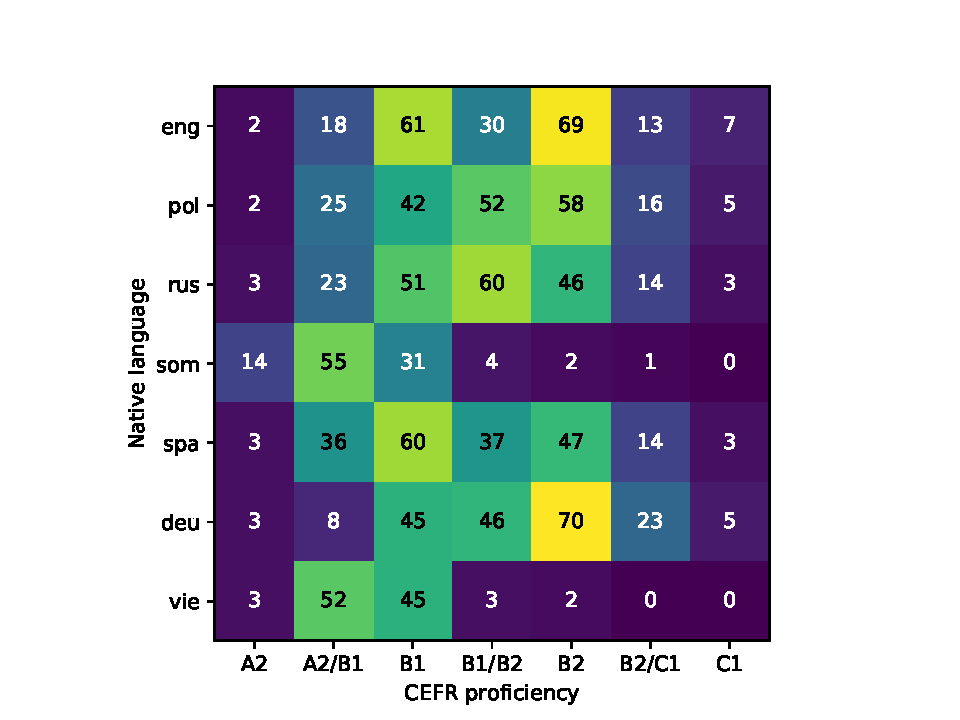
\includegraphics{lang_vs_cefr}
  \caption{The distribution of proficiency scores for each L1}
  \label{fig:lang-vs-cefr}
\end{figure}
 
\begin{figure}
  \centering
  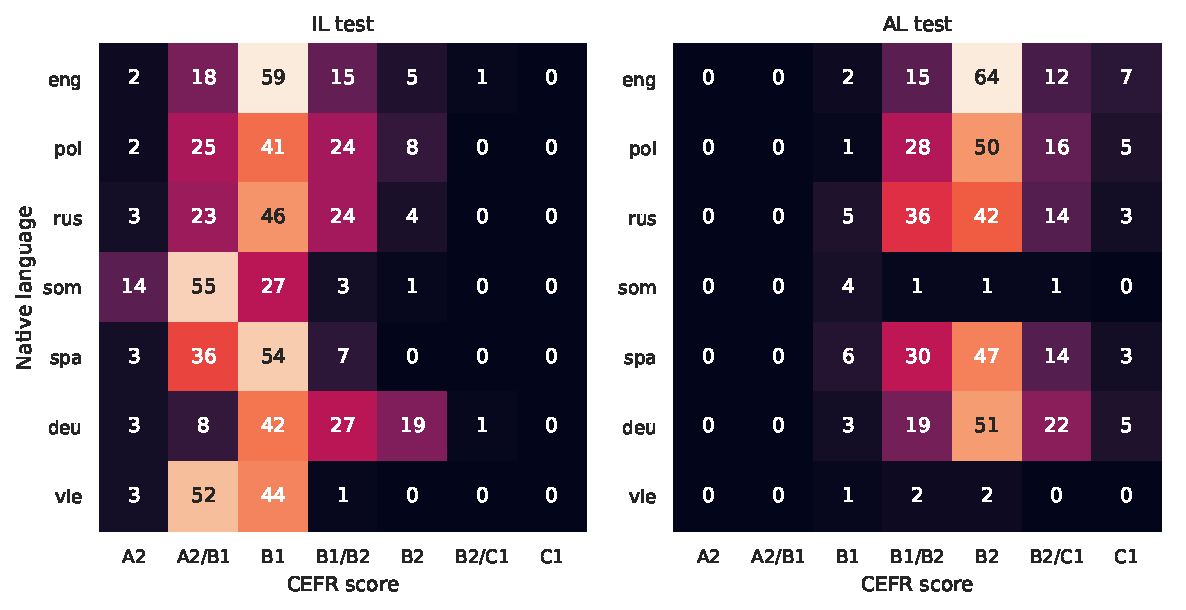
\includegraphics{testlevel_lang_vs_cefr}
  \caption{L1 versus CEFR score for each test level}
  \label{fig:testlevel-lang-vs-cefr}
\end{figure}

We analyze the data set in order to find correlations between different
metadata. Knowing that the documents stem from two different language tests
that measure different levels of proficiency, the data set was split in two
using the \emph{Test level} label, and then broken down by language and
proficiency again. Figure \ref{fig:testlevel-lang-vs-cefr} shows that the
test levels have different distributions of proficiency. Note also that two
language groups are underrepresented at the B2 test level (\emph{AL test}),
namely Somali and Vietnamese, which have seven and five essays in the B2 test
level, respectively. All other combinations of L1 and test level contain
exactly 100 essays. This partly explains the low average proficiency of
Somali and Vietnamese speakers apparent in figure \ref{fig:lang-vs-cefr}. The
difference compared to the other language groups is not as salient when
looking only at the B1 test level (\emph{IL test}) data.

\begin{table}
  \centering
  \begin{tabular}{lrrr}
    \toprule
    Topic                    & AL test & IL test & Total \\
    \midrule
    % cspell:disable
    telefon                  &      37 &      64 &   101 \\
    bolig                    &       0 &      83 &    83 \\
    familie helse vekt       &      59 &       0 &    59 \\
    tid                      &       2 &      51 &    53 \\
    natur norge              &       0 &      48 &    48 \\
    folk relasjoner vennskap &       0 &      45 &    45 \\
    tradisjoner flytting     &       0 &      38 &    38 \\
    barn                     &       3 &      32 &    35 \\
    kultur norge             &       0 &      34 &    34 \\
    media                    &       0 &      31 &    31 \\
    % cspell:enable
    \bottomrule
  \end{tabular}
  \caption[Most common topics in ASK texts]{
    The number of texts in each test level for the top 10 topics
    across test level.
  }
  \label{tab:texts-per-topic}
\end{table}

Another interesting variable is the essay topic. There is generally a strong
correlation between topic and vocabulary, and not accounting for this may
lead to a model picking up the wrong signal. Since the data is collected from
two different language tests, we might expect the distribution of topics to
differ between the test levels, and this is the case. Looking at the ten most
common topics in the data (table \ref{tab:texts-per-topic}), several are only
present on one test level.

There is also a difference in granularity. There are 52 topics in ``Høyere
nivå'' and only 38 topics in \emph{IL test}, even though there are more
documents in the latter test level (512 vs. 700). This also means that the
topics within each test level have different support. The median number of
documents for a topic in \emph{AL test} is 5 (mean $9.8$), while it is 11 in
\emph{IL test} (mean $18.4$). This also explains the overrepresentation of
\emph{IL test} in the table of top ten topics.

% cspell:disable
It has been observed that some topics in the diagram consist of several
sub-topics (for instance, ``natur norge'' consists of ``natur'' and
``norge''). However, the number of individual sub-topics is 62, still quite
large. However, they seem to be more evenly distributed across essays. The
median number of documents for a sub-topic, for both test levels, is 25 (mean
$34.8$). 13 sub-topics are only represented in 5 or fewer documents.
% cspell:enable

\begin{figure}
  \centering
  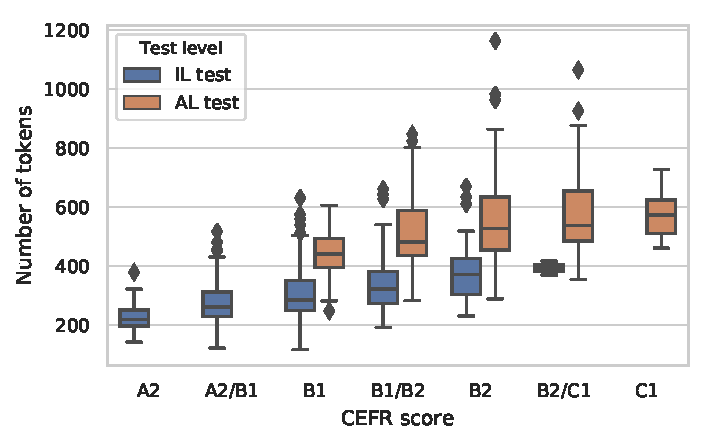
\includegraphics{testlevel_lengths_per_cefr}
  \caption[Document lengths on each CEFR level]{
    Distributions of essay lengths for CEFR scores on each test level.
  }
  \label{fig:testlevel-lengths-per-cefr}
\end{figure}

Document lengths have been seen to correlate with essay score in other
studies such as \textcite{vajjala17}. To see the relationship between these
variables in ASK, we again break down the data into the two test levels. One
group, \emph{B2/C1} CEFR score within \emph{IL test}, was excluded due to
having fewer than ten documents. Looking at figure
\ref{fig:testlevel-lengths-per-cefr}, two relations are apparent. Essays in
the \emph{AL test} test level are generally longer than in \emph{IL test},
and within each test level the higher scoring essays are generally longer.
Also, outliers are generally on the long side.

Note that even for the same CEFR score, the essays from the higher test level
are considerably longer. As an example, consider the \emph{B1/B2} score,
which is the most evenly distributed between the two test levels (101 essays
in \emph{IL test}, 131 in \emph{AL test}). More than 75\% of these texts on
the lower test level have fewer than 400 tokens, and more than 75\% on the
higher level are longer than 400 tokens. In fact, for all four CEFR scores
that are present on both test levels, there is no overlap of the
interquartile ranges\footnote{The range of values when the top 25\% and
bottom 25\% are excluded} between IL and AL test level.


\section{Data split}

At the start of the project, the dataset was split into a training,
development and test set in a 8:1:1 proportion. Ideally, the train and test
sets would have the same distribution of classes, but the limited amount of
data made this more difficult. As can be seen from figure
\ref{fig:lang-vs-cefr}, 15 of the combinations language vs. proficiency label
consist of only three or fewer documents.

Moreover, we wanted each split to consist of text topics not present in the
other splits. The reason for this to prevent a model from learning a bias for
topic. Finding a split that satisfies our constraints is an optimization
problem for which it can be intractable to find an optimal solution. We
therefore turned to heuristics, hoping that it would help us find a good
local optimum.
 
The split was chosen in order to have the right proportion of documents in
each part of the split, and so the distribution of proficiency and native
language is as similar as possible across the separate parts of the data
split. Specifically, the split was found by running an evolutionary algorithm
with a fitness function favouring splits that were as close as possible to
8:1:1 in proportion, while ensuring that each split contained a disjoint set
of topics.

We designed a fitness function incurred several penalties. A candidate split
was given a size penalty proportional to the absolute difference between the
sizes of test and dev splits and the wanted size, namely 10\% of the corpus.
Further, we added a label distribution penalty by calculating the
Kullback-Leibler divergences between the distributions of CEFR and L1 labels
in the candidate splits and the distribution in the entire corpus.
Kullback-Leibler divergence was computed using the SciPy \autocite{scipy}
library. The divergence values were squared and added to the penalty.

\begin{table}
  \centering
  \begin{tabular}{ll}
    \toprule
    Topics in development set &       Topics in test set \\
    \midrule
    % cspell:disable
         idrett/sport kultur &       geografi norge folk \\
                organisasjon &               innvandring \\
                  opplevelse & innvandring politikk valg \\
                     økonomi &              idrett/sport \\
                    holdning &            bolig geografi \\
           barn idrett/sport &               arbeid yrke \\
            familie flytting &          økonomi holdning \\
               eldre familie &              humor kultur \\
               helse røyking &   politikk norge holdning \\
       litteratur dikt språk &            litteratur bok \\
    helse arbeid innvandring &  familie befolkning norge \\
                barn familie &    litteratur dikt idrett \\
                       helse &           folk utdannelse \\
            utdannelse språk &         politikk holdning \\
          arbeid innvandring &                  media tv \\
      litteratur dikt venner &                  religion \\
                             &               helse organ \\
                             &             folk følelser \\
    % cspell:enable
    \bottomrule
  \end{tabular}
  \caption[Essay topics in development and test sets]{
    The topics chosen to be in each of the development and test sets.
  }
  \label{tab:topics-in-split}
\end{table}

% cspell:disable
The split in terms of the topics can be seen in table
\ref{tab:topics-in-split} \footnote{In the XML files, the topic values
contain a trailing space character, not visible in print.}. The dev and test
sets contain 123 texts each, close to the ideal 10\% of the corpus, which is
121. The topic variable has values which are sets of keywords, and therefore
there is still topical overlap between splits. For example, `økonomi'
(economy) and `økonomi holdning' (economy attitude) are considered separate
values and assigned to different splits, even though both topics include the
`economy' keyword.
% cspell:enable

\begin{figure}
  \centering
  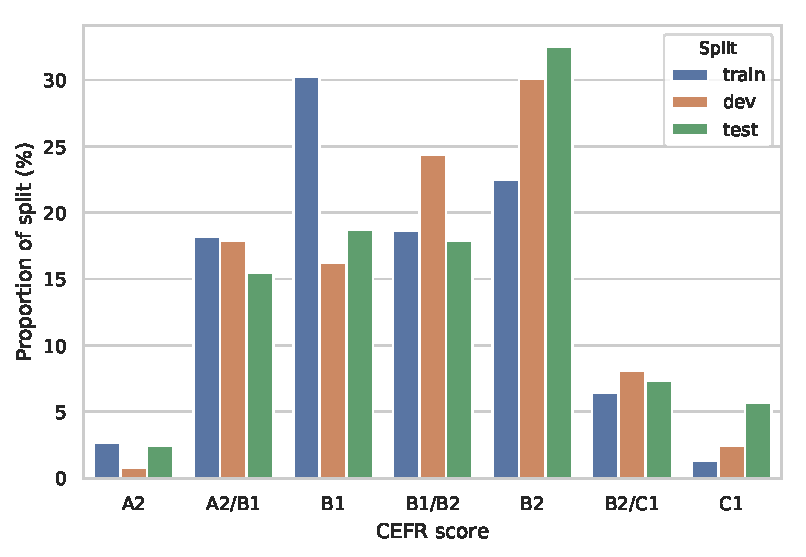
\includegraphics[width=\textwidth]{split-cefr-dist}
  \caption{Proportional distribution of CEFR labels in the three splits.}
  \label{fig:split-cefr-dist}
\end{figure}

\begin{figure}
  \centering
  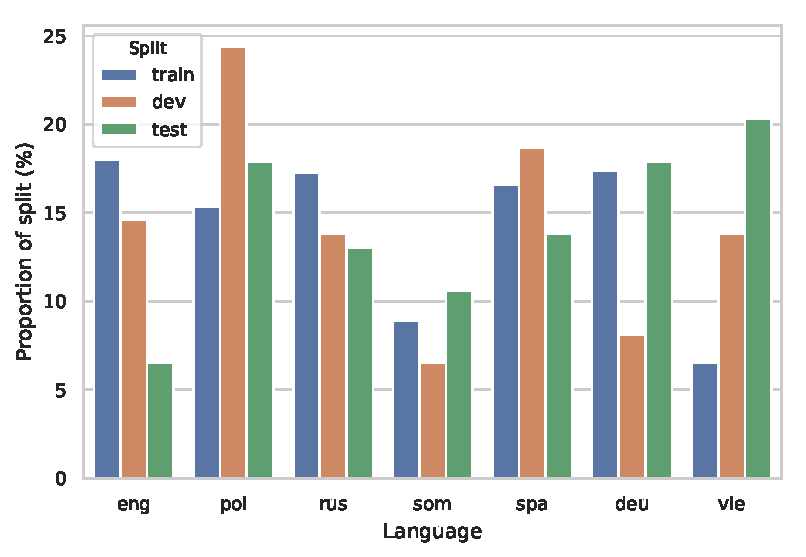
\includegraphics[width=\textwidth]{split-lang-dist}
  \caption{Proportional distribution of language labels in the three splits.}
  \label{fig:split-lang-dist}
\end{figure}

Figure \ref{fig:split-cefr-dist} shows how CEFR labels are distributed in the
resulting training, development and test splits, and figure
\ref{fig:split-lang-dist} shows the same for language labels. It can be seen
that all splits contain texts on all CEFR levels and for all different
\acp{L1}. While there are considerable differences in the distributions, we
decided that the result was reasonable given the constraints and the small
size of the dataset.

Each split does not contain every combination of CEFR score and \ac{L1}. This
follows from the distribution plotted in figure \ref{fig:lang-vs-cefr}, where
we find five combinations of CEFR score and \ac{L1} that occur only once or
twice. Since each document is assigned to exactly one of three different
splits, these combinations must necessarily be absent from one or two of the
splits.



\section{Preprocessing}

The data files in the ASK corpus are in XML format, and contain information
about tags, mistakes and corrections, paragraphs, sentences and more. These
files were transformed into other formats during the process. First, they
were converted to plain text files stripped of all tags or correction labels,
with one sentence per line consisting of space-separated tokens, and an empty
line separating paragraphs.

These raw text files were then sent through the UDPipe pipeline for tagging
and dependency parsing. The output from UDPipe is in the CoNLL file format
with a single token per line. UDPipe tags the documents using the UD tagset,
while the original tags in the XML documents are from the Oslo-Bergen
tagger's own tagset.

\section{Baseline}

A logistic regression classifier was able to predict the CEFR score with
43.9\% accuracy using only two features: The length of the document, in
number of tokens, and the test level (IL test or AL test). 54 of 123
documents in the dev set.

A convolutional neural network based on the architecture in
\textcite{zhang2017sensitivity} achieved an accuracy of 42.3\% using
sequences of POS tags as input to an initial embedding layer.

Note that always predicting the majority class in the dev set (B2 with 37
documents) yields an accuracy of 30.1\%.


\chapter{Convolutional and recurrent neural networks}
\label{ch:sequencemodels}

In the previous chapter we established baseline results for the \ac{AES} task,
and found that for the systems we implemented, regression gave better results
than nominal classification.

We now go on to investigate distributed representations of inputs and more
advanced neural architectures, namely \acp{CNN} and \acp{RNN}. Both
architectures are widely used in various \ac{NLP} tasks. Their advantage is
the ability to automatically extract features that are more domain-specific
than the simple representations we used in chapter \ref{ch:baseline}. For
instance \acp{CNN} can be considered as \ngram detectors. Instead of having
to find and count \ngrams to feed as inputs to the system, the \ac{CNN} can
take a sequence of tokens and find the most informative \ngrams for the task
at hand by end-to-end training\autocite[155]{goldbergNLP}.

Coupled with distributed representations of words, i.e. word embeddings,
similar \ngrams can also share representation. For instance, assuming a
setting where the embeddings for the words `nice' and `good' are similar, the
3-grams `nice to hear' and `good to hear' may be efficiently encoded in a
\ac{CNN}. The features produced by the network are not binary or integer
counts, but real-valued vectors.

The strength of \acp{RNN} is their theoretical ability to detect long range
features. This should intuitively be useful for the tasks at hand. For
instance, discourse features of a text, such as how different sections of a
text are connected and referring to topics that have been mentioned before,
can be considered a part of language proficiency. Learning to build complex
sentences and producing longer discourse is a part of acquiring a second
language.

In the following, we will first describe the experimental setup that is
common for CNN and RNN experiments. We will also describe the pre-trained
word embeddings used in some experiments. CNN and RNN experiments and results
for the \ac{AES} task will be discussed separately. We will also briefly see
how the models perform on the \ac{NLI} task on its own, and visualize some of
the system internals to see if it aids the interpretation of system
performance.


\section{Experimental setup}

As in the last chapter, models are trained on the training set, and we use the
development set as validation data to decide which weights to keep. We keep
the weights that gave the highest macro \FI score over the validation set in
the course of training. The reported metrics are also evaluated on the
development set.

Certain aspects of the experimental setup for the new models are different
from the models in the previous chapter, but shared between \ac{CNN} and
\ac{RNN} models. These aspects are described in this section. Like the
\ac{MLP} models in chapter \ref{ch:baseline}, the neural networks are
implemented in \textcite{keras} and trained on the \textcite{tensorflow}
backend.


\subsection{Input length}

The models in this chapter take as input a document of a predetermined
length. We therefore need to set a fixed number of tokens that will be the
length of each document. Documents shorter than this length were padded to
this length by appending special padding tokens, and longer documents were
truncated. In order to decide this fixed length, we examined the distribution
of document lengths in the training set. All the subsequent values are
rounded to the nearest integer. First, we found the 95th percentile of
document lengths, which turned out to be 701 tokens. Then, we computed a
common threshold for high outliers, the upper quartile plus 1.5 times the
interquartile range:
\[
  Q_3 + 1.5 \cdot (Q_3 - Q_1)
\]
This gives 825 tokens. Finally, we computed the mean value plus two standard
deviations, giving 707 tokens. We decided to settle on 700 tokens as our
document length, since it is a round number close to two of three values we
examined. We know that using this value, a great majority of documents will
not be truncated at all.

As a consequence of the unequal distributions of length between the two test
levels, the documents that are truncated are mainly from the advanced level
test. Thus, the presence of padding tokens at the end is a strong indicator
of a text coming from the AL test. It is potentially problematic that this
truncation only happens to documents from one test level, since the two test
levels are seen to have different distributions of both CEFR scores and
\acp{L1}. Nevertheless, even if truncation did not happen, a model might be
able to discern the test levels just by document length, since we do not hide
the document length from the model.


\subsection{Pre-trained embeddings}
\label{subseq:fasttext}

We experimented with randomly initialized word embedding vectors trained from
scratch, as well as initializing the vectors with pre-trained embeddings. We
know that our corpus contains tokens with spelling mistakes, which are likely
to be absent in any pre-trained vector model. We therefore sought out
pre-trained models using the FastText algorithm, which lets us compute
vectors even for words that do not have separate entries in the model, in
which case the model creates a vector based on the word's constituent
character \ngrams.

In our case, we used a selection of models trained on a large Norwegian
corpus, the combination of Norsk aviskorpus (The Norwegian Newspaper Corpus)
and NoWaC (Norwegian Web As Corpus) \autocite{stadsnes2018}. These vector
models are very large, containing vectors for more than 2,500,000 words. The
models are stored in a repository that is available online and on the Abel
supercomputer cluster \autocite{murhaf2017repository}. We use three models
trained on this corpus using the FastText algorithm, differing only in the
dimension of embeddings. They were trained using skipgram and window size 5, 
and lemmatization has not been applied to the corpora.

We can superficially confirm the usefulness of FastText embeddings by looking
at vector similarities. We use the Python library Gensim \autocite{gensim} to
load vector models and look up word similarities. For instance, the token
`kjokoladet' is a misspelt version of `sjokolade' (chocolate), and it is
closest in the embedding space to `sjokolade'. Curiously, it is also closer
to `potetgul' than `potetgull' (potato crisps), where the former is a
misspelling.

Our training data only contains 20,766 unique tokens, which is less than 1\%
of the full vocabulary of the models. Loading the full pre-trained model
takes a long time and uses huge amounts of memory for word vectors we will
never use. For that reason, we created models of smaller size by loading the
full models once and iterating through all of the word forms in our corpus,
storing the resulting vectors in a new vector model containing only 20,766
words. In this way, we are also able to benefit from the FastText models'
ability to compute vectors for unknown words, since the \ngram algorithm is
being used when computing the reduced models. However, after the embedding
layers of our models have been initialized with vectors from the FastText
model, fine-tuning of vectors happens in the same way as if we had used
embeddings from any other model such as Word2vec, or even randomly
initialized embeddings, since the FastText network is not incorporated into
our models.

Two common variations on training a neural model with pre-trained word
embeddings are using dynamic embeddings, where the embedding vectors are
updated by gradient descent as part of training the entire network, and
static embeddings, where the embedding vectors are kept constant while other
weights in the network are updated. Additional variations are also found in
literature, for example the multi-channel approach seen in
\textcite{kim2014convolutional} where two embedding layers, one static and
one dynamic, are run in parallel. In this study we will not use static
embeddings, but always fine-tune our embeddings, whether they are pre-trained
or randomly initialized.

Experiments using mixed UPOS tags as input will not use pre-trained
embeddings. This is because of two reasons. First, we do not have any
pre-trained embeddings for UPOS tags. Second, the pre-trained word embeddings
for function words that occur in the mixed UPOS tag representation are
trained in the context of content words, and we therefore do not expect them
to have much utility in the context of UPOS tags.


\subsection{Multi-channel input}

In some of our experiments we use both word tokens and their POS tags as
input at the same time. To do this we include two separate embedding matrices
in our network, one for words and one for POS tags. These embedding matrices
do not have to be of the same dimensions, and since the number of different
POS tags is very low compared to the number of different words, we use
smaller vectors for POS tags.

To create the input to the core part of our network, we concatenate the word
and POS embeddings into a single vector. For instance, if we use word
embeddings of size 100 and POS embeddings of size 10, the next layer will
receive vectors of size 110. To implement this, we create two separate
embedding layers in Keras. One for words, which has embedding dimension 100,
and one for UPOS tags, which has embedding dimension 10. Then, we use a
concatenation layer to combine these two layers, and get a layer with vector
size 110.
\todo{implementation details, keras etc}


\section{Convolutional neural networks}

We create a system with a convolutional architecture based on the model
described in \textcite{kim2014convolutional}. Documents are represented as
sequences of token IDs, and fed into an embedding lookup layer. A separate
token ID is used for padding if the document is shorter than 700 tokens.
Another unique token ID is used for unknown tokens, i.e. tokens that either
are not present in training data, or are not among the $n$ most frequent
tokens, if we select a frequency cut-off.

The central part of the architecture is a set of convolutional filter banks
that are applied to sequences of embeddings. We may use several different
window sizes for the filters. The default architecture from
\textcite{kim2014convolutional} uses 300 convolutional filters: 100 each of
window size 3, 4 and 5. After applying the convolutions, the output is max
pooled along the time axis. This selects the highest output of each filter
computed across all windows in the document. In practice, three pooling
operations are included in the computational graph, one for each filter bank.
This is a technical consideration, necessary because of the different window
sizes.

The pooled vectors for each of the filter banks are concatenated into a
single vector, representing the document as a whole. This vector has as many
elements as there are filters in all the filter banks combined. This
representation vector is fed to a final softmax layer to produce a
classification output. During training, we apply dropout to this final weight
layer as a regularization method. The last dense layer uses dropout with
$p=0.5$ and a constraint on maximum $L_2$ norm of 3.\todo{check}

We do not make any changes to the core of the
\citeauthor{kim2014convolutional} architecture, but we experiment with
different output layers and input representations. Filters of size 3, 4, and
5 were used.


\subsection{Results}

Table \ref{tab:cnn-results} presents the \FI scores on the \ac{AES} task from
our \ac{CNN} experiments. The best macro \FI score on the full set of labels
is a regressor using mixed UPOS input ($0.258$). The second best results comes
from a regressor initialized with pre-trained embeddings. This is also the
model with the highest macro \FI on the collapsed labels. \todo{incomplete}

\begin{table}
  \centering
  \begin{tabular}{lrrrr}
    \toprule
      & \multicolumn{2}{c}{All labels}   & \multicolumn{2}{c}{Collapsed labels} \\
    \cmidrule(lr){2-3}
    \cmidrule(lr){4-5}
    Model   & Macro \FI   & Micro \FI   & Macro \FI   & Micro \FI \\
    \midrule
    \multicolumn{5}{c}{Randomly initialized embeddings} \\
    \midrule
    % $BEGIN autotable cnn-results
    % $META models-per-row=2 columns-per-model=macrof1,microf1
    % $ROW CNN:             cnn-26515464_1    cnn-26518498_1
    % $ROW CNN+POS:         cnn-26515464_2    cnn-26518498_2
    % $ROW CNN Mix:         cnn-26515464_3    cnn-26518498_3
    % $ROW CNN Reg:         cnn-26515464_4    cnn-26518498_4
    % $ROW CNN Reg+POS:     cnn-26515464_5    cnn-26518498_5
    % $ROW CNN Reg Mix:     cnn-26515464_6    cnn-26518498_6
    % $ROW CNN Rank:        cnn-26515464_7    cnn-26518498_7
    % $ROW CNN Rank+POS:    cnn-26515464_8    cnn-26518498_8
    % $ROW CNN Rank Mix:    cnn-26515464_9    cnn-26518498_9
    %\midrule \multicolumn{5}{c}{Pre-trained, fine tuned embeddings} \\ \midrule
    % $ROW CNN:             cnn-26515464_10   cnn-26518498_10
    % $ROW CNN+POS:         cnn-26515464_11   cnn-26518498_11
    % $ROW CNN Reg:         cnn-26515464_13   cnn-26518498_12
    % $ROW CNN Reg+POS:     cnn-26515464_14   cnn-26518498_13
    % $ROW CNN Rank:        cnn-26515464_16   cnn-26518498_14
    % $ROW CNN Rank+POS:    cnn-26515464_17   cnn-26518498_15
    % $END autotable
    CNN & $0.168$ & $\mathbf{0.398}$ & $0.388$ & $0.732$ \\
    CNN+POS & $0.146$ & $0.374$ & $0.398$ & $0.748$ \\
    CNN Mix & $0.201$ & $\mathbf{0.398}$ & $0.383$ & $0.724$ \\
    CNN Reg & $0.230$ & $0.382$ & $0.439$ & $0.724$ \\
    CNN Reg+POS & $0.236$ & $0.341$ & $0.383$ & $0.724$ \\
    CNN Reg Mix & $\mathbf{0.258}$ & $\mathbf{0.398}$ & $0.412$ & $0.642$ \\
    CNN Rank & $0.177$ & $0.374$ & $0.392$ & $0.740$ \\
    CNN Rank+POS & $0.187$ & $0.382$ & $0.397$ & $0.748$ \\
    CNN Rank Mix & $0.231$ & $0.382$ & $0.379$ & $0.715$ \\
    \midrule
    \multicolumn{5}{c}{Pre-trained, fine tuned embeddings} \\
    \midrule
    CNN & $0.208$ & $0.382$ & $0.384$ & $0.724$ \\
    CNN+POS & $0.161$ & $0.366$ & $0.402$ & $\mathbf{0.756}$ \\
    CNN Reg & $0.242$ & $0.341$ & $\mathbf{0.463}$ & $0.724$ \\
    CNN Reg+POS & $0.232$ & $0.366$ & $0.411$ & $0.715$ \\
    CNN Rank & $0.198$ & $0.350$ & $0.384$ & $0.724$ \\
    CNN Rank+POS & $0.181$ & $0.325$ & $0.401$ & $\mathbf{0.756}$ \\
    \bottomrule
  \end{tabular}
  \caption[\FI scores of CNN classifiers on AES.]{
    \FI scores of CNN classifiers on AES. +POS: Multi-channel input with
    both words and UPOS tags. Reg: Regression model. Rank: Ordinal regression.
  }
  \label{tab:cnn-results}
\end{table}


\subsubsection{Comparing classification, regression and ordinal regression}

Comparing the different prediction methods, namely categorical
classification, numeric regression and ordinal regression, we see that
numeric regression overall has the highest macro \FI scores. This is similar
to the observations we made in the previous chapter. Based on this, we
decided to stick to neural regression models only in the next section, where
we train \ac{RNN} models.


\subsection{Training behaviour}

\begin{figure}
  % cnn-26515464_6
  \begin{subfigure}{\linewidth}
    \centering
    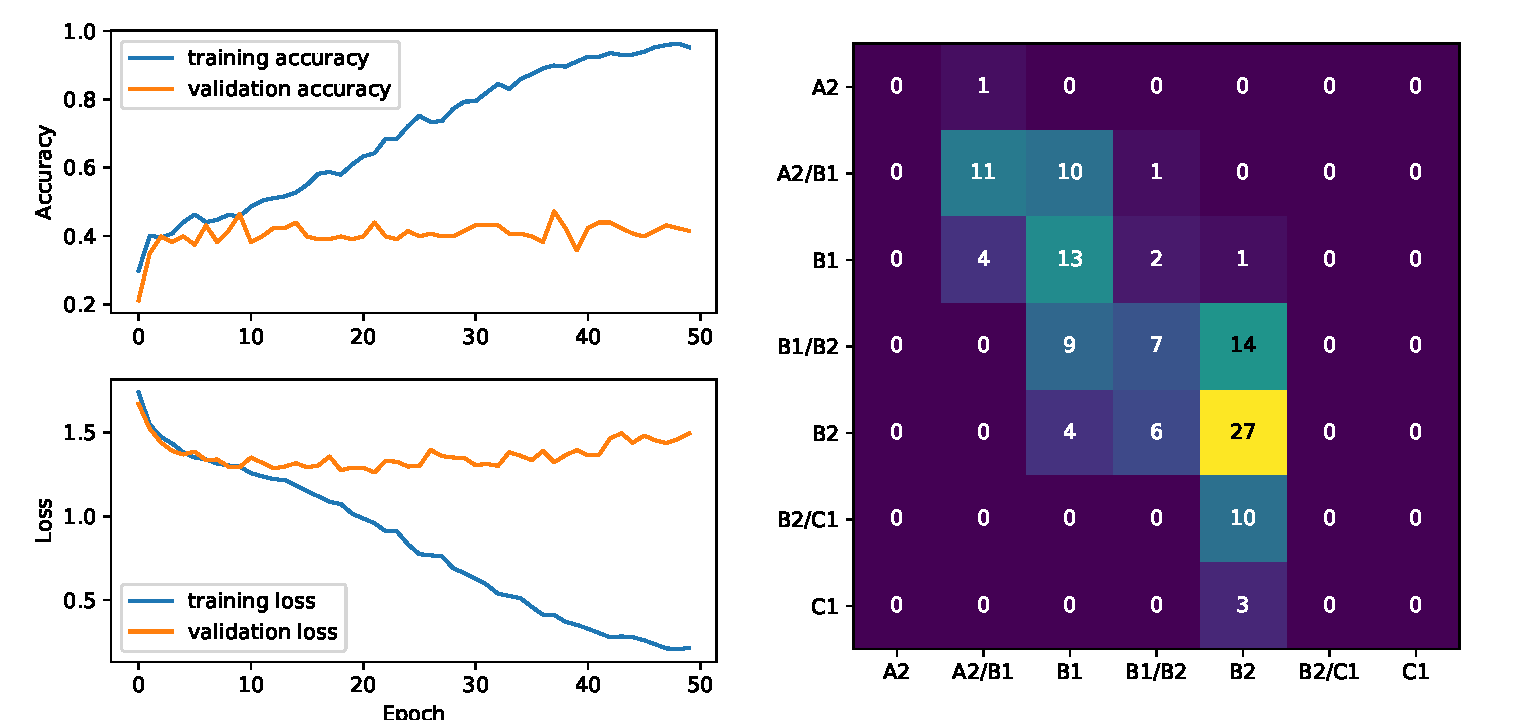
\includegraphics{cnn-training}
    \caption{
      Training and validation loss and validation F1 over 50 epochs of
      training.
    }
  \end{subfigure}
  \begin{subfigure}{\linewidth}
    \centering
    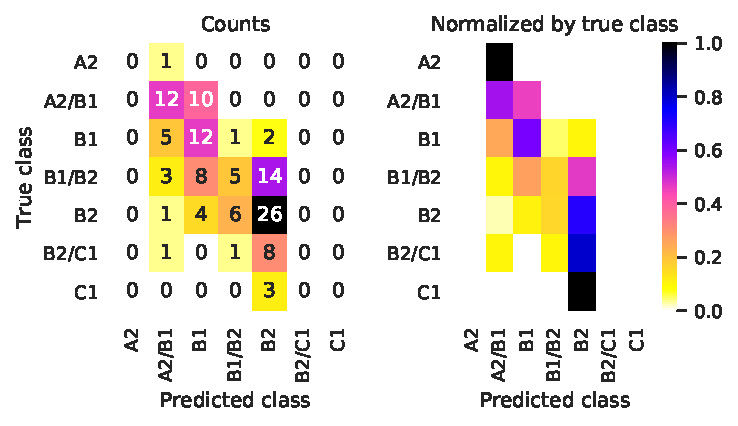
\includegraphics{cnn-confusion}
    \caption{
      Confusion matrix on validation set, raw counts and normalized.
    }
  \end{subfigure}
  \caption[Training behaviour of CNN regression]{
    CNN regressor with mixed UPOS tags as input.
  }
  \label{fig:cnn-training}
\end{figure}

Figure \ref{fig:cnn-training} shows how the training and validation metrics
evolve in the course of training, as well as the confusion matrix of the
final model's predictions. While the training loss quickly converges to a
very low value, the validation loss fluctuates around a much higher loss,
indicating overfitting. The plot of validation macro \FI also shows large
fluctuations.

The confusion matrix reveals that the final model did not assign any samples
to the classes `A2', and `C1', the peripheral classes which are also the
smallest in the validation set. As noted in the discussion about metrics in
the previous chapter (\ref{metrics-discussion}), classes with no predictions
contribute to a low macro \FI score.

Overall, the convolutional models were not able to improve on the macro or
micro \FI scores the \ac{MLP} models in the previous chapter achieved.
However, while the \ac{MLP} confusion matrix (fig. \ref{fig:mlp-char-rank})
had several predictions scattered away from the diagonal, the confusion
matrix for the \ac{CNN} looks like a fuzzy diagonal line, with gradual
dropoff as the distance from the diagonal increases. It also looks like it
has a steeper slope than the ideal diagonal running between the top-left and
bottom-right corner, which is not ideal, but even if the slope is wrong, a
diagonal indicates that relative ranks between essays are reasonable.

We wondered whether the visible difference between scattered predictions and
a fuzzy diagonal could be explained using other metrics than macro or micro
\FI, on which we have previously decided to base our model evaluations. We
therefore collected additional metrics for the best MLP model from the
previous chapter, as well as the best CNN model in this chapter. The results
are listed in table \ref{tab:mlp-cnn-metrics}. We observe that though the
\ac{MLP} has the best \FI scores, the \ac{CNN} beats it in terms of ranking
and error metrics. This explains the intuition of the CNN confusion matrix
looking better\todo{wording}.

It is worth noting that CNN Reg Mix has 149,101 trainable parameters, compared
to the 2,032,206 of MLP Rank char, which is more than 13 times as many.\todo{what to conclude}

\begin{table}
  \centering
  \begin{tabular}{lrr}
    \toprule
    Metric                       & MLP Rank Char & CNN Reg Mix \\
    \midrule
    Macro \FI                     & $\mathbf{0.330}$ & $0.258$ \\
    Micro \FI                     & $\mathbf{0.480}$ & $0.398$ \\
    Spearman's ranked correlation & $0.580$ & $\mathbf{0.647}$ \\
    Mean absolute error           & $0.805$ & $\mathbf{0.756}$ \\
    Root mean squared error       & $1.24$  & $\mathbf{1.03}$ \\
    \bottomrule
  \end{tabular}
  \caption[Comparison of metrics for a MLP and a CNN model]{
    Metrics for MLP Rank Char and CNN Reg Mix. For error metrics, lower values
    are better.
  }
  \label{tab:mlp-cnn-metrics}
\end{table}


\section{Recurrent neural networks}

\todo{describe t\&n model}
Next, we move to a different kind of architecture, \acp{RNN}. We implemented
several models that were variants of the architecture described in
\textcite{taghipour16}. The various changes we made to their architecture
are described below. Some of our variations are similar to the variations
in \textcite{taghipour16}, while others are different ideas. There are also
variations from the paper that we do not implement ourselves, such as a
combined \ac{RNN} and \ac{CNN} model.

We explore some variations in hyperparameters, namely LSTM vs. GRU cells,
unidirectional networks vs. BiRNN, different input representations, different
pooling methods, and compare random initialization of the embedding layer
with using pre-trained vectors.

The embedding layer in \textcite{taghipour16} was of dimension 50 and
randomly initialized. We increased the embedding dimension to 100, and
experimented both with randomly initialized embeddings and with pre-trained
ones.

We are reporting macro and micro \FI as before, not QWK as
\citeauthor{taghipour16}. Refer to section \ref{metrics-discussion} for the
discussion of different metrics for the task.

The ASAP data that \citeauthor{taghipour16} use consists of essays from eight
different prompts, and the range of scores differs across prompts. Since the
scores are numeric values over different ranges, modelling the task as a
regression problem made it sufficient to normalize the numeric scores to a
common interval before training.

Unlike our corpus, ASK, the ASAP dataset used by \citeauthor{taghipour16}
contained essays that were not necessarily written in a second language. Our
data is not split into different parts based on the prompt. There are two
different test levels in ASK, but these are not distinguished in training.


\subsection{Variants}

We create \acp{RNN} with two different types of gated \ac{RNN} cell, the
\ac{LSTM} and the \ac{GRU}. The concept of gated cells is explained in
section \ref{seq:rnn}, along with the equations defining the gated cells. In
Keras, the default activation function for the gates in gated RNNs is the
\emph{Hard sigmoid} activation function (ref. eq. \ref{eq:hardsigmoid}),
chosen because it is computationally more efficient than the sigmoid
function.

We attempted three different pooling methods, that is, ways of combining a
sequence of hidden states from the \ac{RNN} into a feature vector. The first
approach is \emph{mean over time}, where we apply element-wise, unweighted
averaging to the RNN output across the time dimension. This means that the
first element of the representation vector is the average of the first
element of the RNN output across time, and similarly for the second element,
etc., as in the following equation:

\[
  \mathrm{mean/time}(x_i) = \frac{1}{T}\sum_{t=0}^T o_{t,i}
\]

where $T$ is the total number of time steps, and $o_{t,i}$ is the output of
the RNN at time step $t$ and index $i$.

The second method is similar to the first, except that the averaging
operation is replaced by a max operation. Each dimension of the vector is the
highest value the hidden state had at that dimension across the entire
sequence. We refer to this as the \emph{max over time}, and it is defined by
the following equation:

\[
  \mathrm{max/time}(x_i) = \max_{t=0}^T o_{t,i}
\]

The final method we used is an attention layer, which differs from the mean
over time layer in that time steps are weighted by an attention mechanism: a
single-layer neural network computes a value between -1 and 1 for each time
step. These values are normalized across all time steps by a softmax layer,
and then used to compute the weighted average.

Since each time step contributes to the final representation in differing
amounts, the mechanism should be able in theory to focus on crucial
information by choosing weights such as to disregard uninformative time
steps, improving performance. The attention mechanism is trained along with
the rest of the network.

The bidirectional models (BiRNN) are constructed by running two \acp{RNN}
over the same input, but in opposite directions. The output from the BiRNN
layer is a sequence of vectors where, for each time step $j$, the vector is
the concatenation of two vectors $[s_f;s_b]$ where $s_f$ at time step $j$ is
the output from the forwards \ac{RNN} after processing the inputs $(x_1, x_2,
\ldots, x_j)$ and $s_b$ the output from the backwards \ac{RNN} after
processing the inputs $(x_m, x_{m-1}, \ldots, x_j)$, where $m$ is the total
number of time steps. The BiRNN should therefore be able to extract context
on both sides of a input time step.

All the models have a hidden state vector of size 300 in unidirectional
\acp{RNN}, and 600 in BiRNNs (300 in each direction). We use all tokens in
the training set as our lexicon, giving a vocabulary size of 20,068 (20,066
unique tokens occurring in the training set, plus two tokens for padding and
unknown words). This entails that the unknown token will receive no training
signal, and its embedding will remain whatever it was initialized as.
Depending on whether the experiment uses pre-trained embeddings, this
representation will either be a random vector, or the embedding computed by
the FastText model for the token `\_\_UNK\_\_'. \todo{sanity - where wat}

Embeddings are initialized either randomly or using vectors
from the FastText model described in section \ref{subseq:fasttext}, and
trained as part of the network. BiRNNs are referred to in the following
tables and discussion as either BiLSTM or BiGRU, depending on the RNN cell
used.


\section{Results}

The RNN results are split into two tables. Table \ref{tab:lstm-results}
contains the results for models with \ac{LSTM} cells, while table
\ref{tab:gru-results} contains the results for models with \ac{GRU} cells.
The mixed input format is only listed in the sections with randomly
initialized embeddings, as it is not applicable when using pre-trained
embeddings.

\begin{table}
  \centering
  \begin{tabular}{lrrrr}
    \toprule
            & \multicolumn{2}{c}{All labels} & \multicolumn{2}{c}{Collapsed labels} \\
    \cmidrule(lr){2-3}
    \cmidrule(lr){4-5}
    Model     & Macro \FI      & Micro \FI      & Macro \FI      & Micro \FI \\
    \midrule
              \multicolumn{5}{c}{Random init, unidirectional LSTM} \\
    \midrule
    % $BEGIN autotable lstm-results
    % $META models-per-row=2 columns-per-model=macrof1,microf1
    % $ROW Mean:        rnn-26519203_1       rnn-26519204_1
    % $ROW Max:         rnn-26519203_2       rnn-26519204_2
    % $ROW Attn.:        rnn-26519203_3       rnn-26519204_3
    % $ROW +POS Mean:   rnn-26519203_4       rnn-26519204_4
    % $ROW +POS Max:    rnn-26519203_5       rnn-26519204_5
    % $ROW +POS Attn:   rnn-26519203_6       rnn-26519204_6
    % $ROW Mix Mean:    rnn-26519203_7       rnn-26519204_7
    % $ROW Mix Max:     rnn-26519203_8       rnn-26519204_8
    % $ROW Mix Attn:    rnn-26519203_9       rnn-26519204_9
    % \midrule \multicolumn{5}{c}{Random init, BiLSTM} \\ \midrule
    % $ROW Mean:        rnn-26530015_10      rnn-26530016_10
    % $ROW Max:         rnn-26530015_11      rnn-26530016_11
    % $ROW Attn:        rnn-26530015_12      rnn-26530016_12
    % $ROW +POS Mean:   rnn-26530015_13      rnn-26530016_13
    % $ROW +POS Max:    rnn-26530015_14      rnn-26530016_14
    % $ROW +POS Attn:   rnn-26530015_15      rnn-26530016_15
    % $ROW Mix Mean:    rnn-26530015_16      rnn-26530016_16
    % $ROW Mix Max:     rnn-26530015_17      rnn-26530016_17
    % $ROW Mix Attn:    rnn-26530015_18      rnn-26530016_18
    % \midrule \multicolumn{5}{c}{Pre-trained, unidirectional LSTM} \\ \midrule
    % $ROW Mean:        rnn-26519203_19      rnn-26519204_19
    % $ROW Max:         rnn-26519203_20      rnn-26519204_20
    % $ROW Attn:        rnn-26519203_21      rnn-26519204_21
    % $ROW +POS Mean:   rnn-26519203_22      rnn-26519204_22
    % $ROW +POS Max:    rnn-26519203_23      rnn-26519204_23
    % $ROW +POS Attn:   rnn-26519203_24      rnn-26519204_24
    % \midrule \multicolumn{5}{c}{Pre-trained, BiLSTM} \\ \midrule
    % $ROW Mean:        rnn-26530015_25      rnn-26530016_25
    % $ROW Max:         rnn-26530015_26      rnn-26530016_26
    % $ROW Attn:        rnn-26530015_27      rnn-26530016_27
    % $ROW +POS Mean:   rnn-26530015_28      rnn-26530016_28
    % $ROW +POS Max:    rnn-26530015_29      rnn-26530016_29
    % $ROW +POS Attn:   rnn-26530015_30      rnn-26530016_30
    % $END autotable
    Mean & $0.268$ & $0.398$ & $0.458$ & $0.675$ \\
    Max & $0.235$ & $0.350$ & $0.475$ & $0.740$ \\
    Attn. & $0.445$ & $0.431$ & $0.624$ & $0.780$ \\
    +POS Mean & $0.251$ & $0.358$ & $0.454$ & $0.699$ \\
    +POS Max & $0.187$ & $0.325$ & $0.435$ & $0.715$ \\
    +POS Attn & $0.417$ & $0.390$ & $0.619$ & $0.772$ \\
    Mix Mean & $0.230$ & $0.350$ & $0.396$ & $0.626$ \\
    Mix Max & $0.210$ & $0.415$ & $0.398$ & $0.748$ \\
    Mix Attn & $0.297$ & $0.431$ & $0.576$ & $0.772$ \\
    \midrule \multicolumn{5}{c}{Random init, BiLSTM} \\ \midrule
    Mean & $0.262$ & $0.366$ & $0.457$ & $0.699$ \\
    Max & $0.182$ & $0.358$ & $0.485$ & $0.724$ \\
    Attn & $\mathbf{0.448}$ & $0.447$ & $0.699$ & $0.805$ \\
    +POS Mean & $0.337$ & $0.333$ & $0.441$ & $0.691$ \\
    +POS Max & $0.176$ & $0.350$ & $0.460$ & $0.715$ \\
    +POS Attn & $0.420$ & $0.407$ & $0.670$ & $0.789$ \\
    Mix Mean & $0.220$ & $0.309$ & $0.402$ & $0.659$ \\
    Mix Max & $0.190$ & $0.374$ & $0.400$ & $0.756$ \\
    Mix Attn & $0.305$ & $0.447$ & $0.550$ & $0.724$ \\
    \midrule \multicolumn{5}{c}{Pre-trained, unidirectional LSTM} \\ \midrule
    Mean & $0.266$ & $0.374$ & $0.443$ & $0.675$ \\
    Max & $0.181$ & $0.358$ & $0.433$ & $0.756$ \\
    Attn & $0.410$ & $0.423$ & $0.626$ & $0.789$ \\
    +POS Mean & $0.280$ & $0.390$ & $0.465$ & $0.691$ \\
    +POS Max & $0.206$ & $0.415$ & $0.414$ & $0.780$ \\
    +POS Attn & $0.370$ & $0.382$ & $0.680$ & $\mathbf{0.813}$ \\
    \midrule \multicolumn{5}{c}{Pre-trained, BiLSTM} \\ \midrule
    Mean & $0.263$ & $0.374$ & $0.470$ & $0.683$ \\
    Max & $0.190$ & $0.325$ & $0.396$ & $0.748$ \\
    Attn & $0.429$ & $\mathbf{0.463}$ & $0.638$ & $0.805$ \\
    +POS Mean & $0.257$ & $0.350$ & $0.465$ & $0.691$ \\
    +POS Max & $0.181$ & $0.358$ & $0.412$ & $0.715$ \\
    +POS Attn & $0.427$ & $0.423$ & $\mathbf{0.704}$ & $0.780$ \\
    \bottomrule
  \end{tabular}
  \caption{\FI scores of LSTM classifiers on AES}
  \label{tab:lstm-results}
\end{table}

\begin{table}
  \centering
  \begin{tabular}{lrrrr}
    \toprule
            & \multicolumn{2}{c}{All labels} & \multicolumn{2}{c}{Collapsed labels} \\
    \cmidrule(lr){2-3}
    \cmidrule(lr){4-5}
    Model     & Macro \FI      & Micro \FI      & Macro \FI      & Micro \FI \\
    \midrule
              \multicolumn{5}{c}{Random init, unidirectional GRU} \\
    \midrule
    % $BEGIN autotable gru-results
    % $META models-per-row=2 columns-per-model=macrof1,microf1
    % $ROW Mean:        rnn-26536430_1       rnn-26536431_1
    % $ROW Max:         rnn-26536430_2       rnn-26536431_2
    % $ROW Attn:        rnn-26536430_3       rnn-26536431_3
    % $ROW +POS Mean:   rnn-26536430_4       rnn-26536431_4
    % $ROW +POS Max:    rnn-26536430_5       rnn-26536431_5
    % $ROW +POS Attn:   rnn-26536430_6       rnn-26536431_6
    % $ROW Mix Mean:    rnn-26536430_7       rnn-26536431_7
    % $ROW Mix Max:     rnn-26536430_8       rnn-26536431_8
    % $ROW Mix Attn:    rnn-26536430_9       rnn-26536431_9
    % \midrule \multicolumn{5}{c}{Random init, BiGRU} \\ \midrule
    % $ROW Mean:        rnn-26536430_10      rnn-26536431_10
    % $ROW Max:         rnn-26536430_11      rnn-26536431_11
    % $ROW Attn:        rnn-26536430_12      rnn-26536431_12
    % $ROW +POS Mean:   rnn-26536430_13      rnn-26536431_13
    % $ROW +POS Max:    rnn-26536430_14      rnn-26536431_14
    % $ROW +POS Attn:   rnn-26536430_15      rnn-26536431_15
    % $ROW Mix Mean:    rnn-26536430_16      rnn-26536431_16
    % $ROW Mix Max:     rnn-26536430_17      rnn-26536431_17
    % $ROW Mix Attn:    rnn-26536430_18      rnn-26536431_18
    % \midrule \multicolumn{5}{c}{Pre-trained, unidirectional GRU} \\ \midrule
    % $ROW Mean:        rnn-26536430_19      rnn-26536431_19
    % $ROW Max:         rnn-26536430_20      rnn-26536431_20
    % $ROW Attn:        rnn-26536430_21      rnn-26536431_21
    % $ROW +POS Mean:   rnn-26536430_22      rnn-26536431_22
    % $ROW +POS Max:    rnn-26536430_23      rnn-26536431_23
    % $ROW +POS Attn:   rnn-26536430_24      rnn-26536431_24
    % \midrule \multicolumn{5}{c}{Pre-trained, BiGRU} \\ \midrule
    % $ROW Mean:        rnn-26536430_25      rnn-26536431_25
    % $ROW Max:         rnn-26536430_26      rnn-26536431_26
    % $ROW Attn:        rnn-26536430_27      rnn-26536431_27
    % $ROW +POS Mean:   rnn-26536430_28      rnn-26536431_28
    % $ROW +POS Max:    rnn-26536430_29      rnn-26536431_29
    % $ROW +POS Attn:   rnn-26536430_30      rnn-26536431_30
    % $END autotable
    Mean & $0.264$ & $0.374$ & $0.455$ & $0.675$ \\
    Max & $0.219$ & $0.325$ & $0.487$ & $0.683$ \\
    Attn & $0.434$ & $0.431$ & $\mathbf{0.806}$ & $0.805$ \\
    +POS Mean & $0.348$ & $0.398$ & $0.450$ & $0.642$ \\
    +POS Max & $0.230$ & $0.374$ & $0.500$ & $0.748$ \\
    +POS Attn & $0.434$ & $0.423$ & $0.718$ & $0.813$ \\
    Mix Mean & $0.225$ & $0.333$ & $0.388$ & $0.634$ \\
    Mix Max & $0.200$ & $0.398$ & $0.398$ & $0.756$ \\
    Mix Attn & $0.302$ & $\mathbf{0.455}$ & $0.509$ & $0.780$ \\
    \midrule \multicolumn{5}{c}{Random init, BiGRU} \\ \midrule
    Mean & $0.314$ & $0.333$ & $0.444$ & $0.667$ \\
    Max & $0.160$ & $0.325$ & $0.460$ & $0.691$ \\
    Attn & $0.459$ & $0.447$ & $0.805$ & $0.805$ \\
    +POS Mean & $0.373$ & $0.333$ & $0.425$ & $0.683$ \\
    +POS Max & $0.175$ & $0.309$ & $0.503$ & $0.748$ \\
    +POS Attn & $\mathbf{0.460}$ & $0.447$ & $0.687$ & $\mathbf{0.821}$ \\
    Mix Mean & $0.231$ & $0.350$ & $0.395$ & $0.642$ \\
    Mix Max & $0.200$ & $0.382$ & $0.405$ & $0.764$ \\
    Mix Attn & $0.275$ & $\mathbf{0.455}$ & $0.617$ & $0.707$ \\
    \midrule \multicolumn{5}{c}{Pre-trained, unidirectional GRU} \\ \midrule
    Mean & $0.274$ & $0.366$ & $0.463$ & $0.715$ \\
    Max & $0.185$ & $0.350$ & $0.401$ & $0.756$ \\
    Attn & $0.414$ & $0.431$ & $0.678$ & $0.797$ \\
    +POS Mean & $0.282$ & $0.382$ & $0.477$ & $0.699$ \\
    +POS Max & $0.193$ & $0.382$ & $0.405$ & $0.764$ \\
    +POS Attn & $0.409$ & $0.423$ & $0.746$ & $0.789$ \\
    \midrule \multicolumn{5}{c}{Pre-trained, BiGRU} \\ \midrule
    Mean & $0.266$ & $0.390$ & $0.435$ & $0.707$ \\
    Max & $0.187$ & $0.398$ & $0.393$ & $0.740$ \\
    Attn & $0.454$ & $0.447$ & $0.773$ & $0.797$ \\
    +POS Mean & $0.281$ & $0.382$ & $0.480$ & $0.724$ \\
    +POS Max & $0.183$ & $0.341$ & $0.397$ & $0.748$ \\
    +POS Attn & $0.433$ & $0.439$ & $0.758$ & $0.805$ \\
    \bottomrule
  \end{tabular}
  \caption{\FI scores of GRU classifiers on AES}
  \label{tab:gru-results}
\end{table}


\subsection{The effect of hyperparameters}

\todo{expand}
We choose five different hyperparameters and examine the effect each of them
has on the predictions of the networks. When it is relevant, we will compare
the effect we got with the effect found by \textcite{taghipour16}. However,
our experiments for many reasons not comparable: We use a different dataset
with different labels, a different evaluation metric, and a different
evaluation method (\citeauthor{taghipour16} use 5-fold cross validation),
among other things. \todo{diff datasets never comparable}


\subsubsection{LSTM versus GRU}

GRU comes out on top with somewhat higher macro \FI scores. When ranking all
models by macro \FI score on the full set of labels, the top three places are
taken by GRU models ($0.460$, $0.459$, $0.454$), and the fourth and fifth
places by LSTM models ($0.448$, $0.445$). A GRU model also has the highest
macro \FI on the collapsed labels ($0.805$). The best LSTM macro \FI on
collapsed labels is $0.704$, ranking seventh among all GRU and LSTM
experiments.

We conclude that GRU performs best on the task. An additional benefit of GRU
is that it has fewer parameters and is a little faster in training.


\subsubsection{Bidirectional RNN}

Our top performing models are BiRNNs, and the unidirectional model with the
highest macro \FI on the full set of labels only ranks fifth among all RNN
experiments (macro \FI $0.445$). When comparing models that differ only in
whether they are bidirectional or not, we do not always see that the macro
\FI is higher in the bidirectional model. However, if we only look at the
models which use an attention mechanism, the bidirectional models win in all
but one case. The GRU attention model with mixed UPOS input drops from
$0.320$ to $0.275$. It seems that BiRNNs may be most effective in conjunction
with an attention mechanism, at least on this dataset.


\subsubsection{Initialization of embeddings}

The effects of initialization is not very clear, and in any case mixed. The
best LSTM models used pre-trained embeddings, and the best GRU models used
randomly initialized embeddings. However, the best GRU model with pre-trained
embeddings has a higher macro \FI score than the overall best LSTM model,
$0.454$ and $0.448$ respectively.


\subsubsection{Pooling method}

There are clear differences in the performance of the three pooling method we
have used, mean-over-time, max-over-time and attention. The one that gives
the worst results is max-over-time, which is the only method that ever gives
a macro \FI score less than $0.2$ on the full set of labels, and even the
best run using max pooling has a macro \FI of $0.235$, lower than several CNN
and MLP models trained previously.

Attention comes out as the clear winner of the three pooling methods. It is
the only pooling method that gives macro \FI scores above 40\% in the full
set of classes. At the other end of the scale, max pooling performs worse
than the other two mechanisms in almost every case. Intuitively, it seems
reasonable that max pooling performs poorly on the task. A couple of mistakes
should not count more towards the result than an otherwise consistent level.

The mean-over-time pooling method is somewhere in between, usually giving
macro \FI scores higher than max-over-time and lower than attention.
Interestingly, this is the opposite of what \textcite{taghipour16} found,
even though we are using a very similar network architecture for the same
kind of task. In their case, mean-over-time gave slightly better results than
attention when they compared them (according to the QWK metric).

It can seem promising that the attention mechanism performs well, since it by
design might be able to give more interpretable results than other neural
methods. However, as we will see below (section \ref{subsec:attentionvis}),
it is not apparent that the attention mechanism aids model interpretation in
our case.


\subsubsection{UPOS tags}

The addition of UPOS tags as a side input seems to have variable effect on
the performance. In the LSTM experiments, all the models with an attention
mechanism had a drop in performance when adding the UPOS side input. However,
in the GRU experiments, some models increased their macro \FI when they used
the UPOS side input, including the overall best model, which had a macro \FI
of $0.459$ without UPOS tags and $0.460$ with them. We also see inconsistent
effects when looking at the results on the collapsed labels.

The mixed UPOS input does not measure up in the RNN context, even though it
had the best results in the CNN experiments. The highest macro \FI from an
RNN with mixed UPOS input is $0.305$ on the full set of labels, and $0.617$
on the collapsed set of labels. This is higher than the best results in the
CNN experiments ($0.258$ and $0.463$). It is possible that RNNs are better
able to make use of the greater amount of information present in full lexical
features.


\subsection{Training behaviour}

\begin{figure}
  % rnn-26536430_15
  \begin{subfigure}{\linewidth}
    \centering
    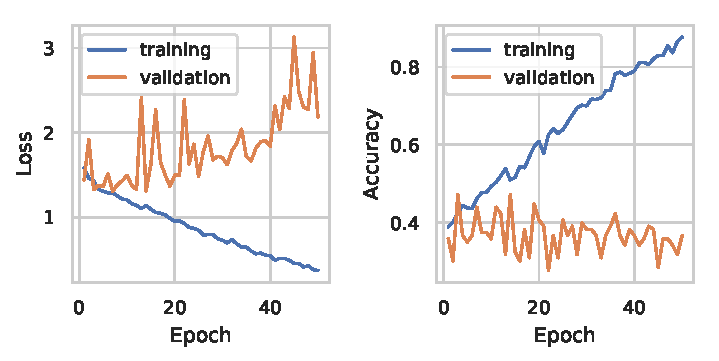
\includegraphics{rnn-training}
    \caption{Training and validation loss and accuracy over 50 epochs of training.}
  \end{subfigure}
  \begin{subfigure}{\linewidth}
    \centering
    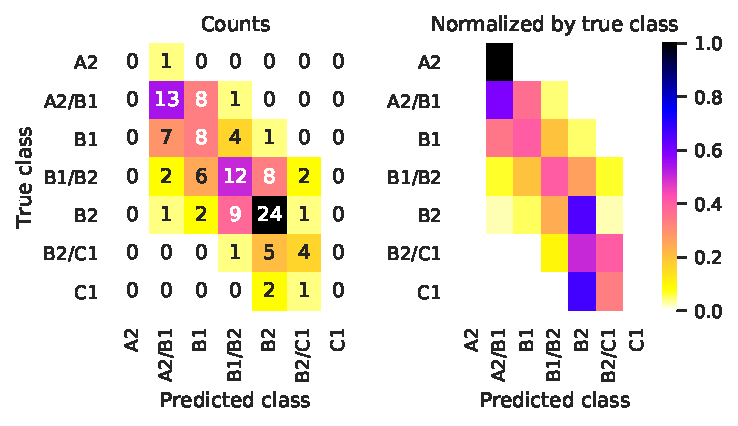
\includegraphics{rnn-confusion}
    \caption{Confusion matrix on validation set, raw counts and normalized.}
  \end{subfigure}
  \caption[Training behaviour of BiGRU with attention]{
    BiRNN with GRU cells, attention mechanism, and pre-trained
    embeddings of dimension 100, fine-tuned.
  }
  \label{fig:rnn-training}
\end{figure}

We see the training and classification of one of the best RNN model in figure
\ref{fig:rnn-training}, a BiGRU model with randomly initialized embeddings
using and an attention mechanism. The plot of the loss shows that the
training loss drops quickly at the beginning and then asymptotically
approaches zero. At the same time, the validation loss quickly converges
around a stable value, but fluctuates somewhat. The plot of macro \FI is more
noisy, with values fluctuating between approximately $0.2$ and $0.4$ for the
entire training process.

We see in the confusion matrix that we can identify a diagonal running from
the top-left to the bottom-right, with zeros in the top-right and bottom-left
corners. We see that mis-classifications are mostly close to the true value,
with only a single prediction being more than two classes away from the gold
label (an instance of `C1' classified as `B1/B2').

Compared to the training plot of the CNN model in figure
\ref{fig:cnn-training}, it seems that the RNN metrics fluctuate much more,
especially on validation data. However, the training accuracy seems to
increase slower, and does not get as close to 100\% in the course of 50 epochs.
\todo{what does this mean}

The BiGRU model has more parameters than the MLP and CNN we looked at before.
The number is 2,817,992.


\section{Native language identification} \label{sec:nli-experiments}

\todo{reintroduce nli ref ch2}
In comparison to proficiency labels in ASK where the peripheral classes are
very small, \acp{L1} are much more evenly distributed. There is also no natural
ordering of \ac{L1}, making regression or ordinal regression pointless. For
experiments in \ac{NLI} we will therefore only use networks with a softmax
classification layer.

We train the same models to classify the documents by native language. The
performance of a \ac{CNN} model improved drastically when including \ac{POS}
tags as input, as evident in table \ref{tab:cnn-nli-results}.

A RNN was able to outperform the CNN only slightly, and here it was not the
attention model that was best, but a bidirectional LSTM.

\begin{table}
  \centering
  \begin{tabular}{lrr}
    \toprule
    Model     & Macro \FI      & Micro \FI \\
    \midrule
    Tokens    &         $0.367$  &         $0.366$  \\ % cnn-nli-2019-02-05_12-54-51
    +POS      & $\mathbf{0.467}$ & $\mathbf{0.463}$ \\ % cnn-nli-2019-01-30_15-32-28
    Mixed POS &         $0.336$  &         $0.333$  \\ % cnn-nli-02-11_16-15-54
    \bottomrule
  \end{tabular}
  \caption{\FI scores of CNN classifiers on NLI}
  \label{tab:cnn-nli-results}
\end{table}

\begin{table}
  \centering
  \begin{tabular}{lrr}
    \toprule
    Model     & Macro \FI      & Micro \FI \\
    \midrule
    % $BEGIN autotable rnn-nli
    % $META models-per-row=1 columns-per-model=macrof1,microf1
    % $ROW Mean:  rnn-nli-26542571_1
    % $ROW Max:  rnn-nli-26542571_2
    % $ROW Attn:  rnn-nli-26542571_3
    % $ROW +POS Mean:  rnn-nli-26542571_4
    % $ROW +POS Max:  rnn-nli-26542571_5
    % $ROW +POS Attn:  rnn-nli-26542571_6
    % \midrule \multicolumn{3}{c}{Random init, BiGRU} \\ \midrule
    % $ROW Mean:  rnn-nli-26542571_7
    % $ROW Max:  rnn-nli-26542571_8
    % $ROW Attn:  rnn-nli-26542571_9
    % $ROW +POS Mean:  rnn-nli-26542571_10
    % $ROW +POS Max:  rnn-nli-26542571_11
    % $ROW +POS Attn:  rnn-nli-26542571_12
    % \midrule \multicolumn{3}{c}{Pre-trained, unidirectional GRU} \\ \midrule
    % $ROW Mean:  rnn-nli-26542571_13
    % $ROW Max:  rnn-nli-26542571_14
    % $ROW Attn:  rnn-nli-26542571_15
    % $ROW +POS Mean:  rnn-nli-26542571_16
    % $ROW +POS Max:  rnn-nli-26542571_17
    % $ROW +POS Attn:  rnn-nli-26542571_18
    % \midrule \multicolumn{3}{c}{Pre-trained, BiGRU} \\ \midrule
    % $ROW Mean:  rnn-nli-26542571_19
    % $ROW Max:  rnn-nli-26542571_20
    % $ROW Attn:  rnn-nli-26542571_21
    % $ROW +POS Mean:  rnn-nli-26542571_22
    % $ROW +POS Max:  rnn-nli-26542571_23
    % $ROW +POS Attn:  rnn-nli-26542571_24
    % $END autotable
    Mean & $0.466$ & $0.480$ \\
    Max & $0.376$ & $0.374$ \\
    Attn & $0.450$ & $0.472$ \\
    +POS Mean & $0.395$ & $0.398$ \\
    +POS Max & $0.346$ & $0.350$ \\
    +POS Attn & $0.412$ & $0.439$ \\
    \midrule \multicolumn{3}{c}{Random init, BiGRU} \\ \midrule
    Mean & $0.471$ & $0.496$ \\
    Max & $0.359$ & $0.382$ \\
    Attn & $0.487$ & $0.463$ \\
    +POS Mean & $0.410$ & $0.423$ \\
    +POS Max & $0.396$ & $0.415$ \\
    +POS Attn & $0.480$ & $0.504$ \\
    \midrule \multicolumn{3}{c}{Pre-trained, unidirectional GRU} \\ \midrule
    Mean & $0.460$ & $0.463$ \\
    Max & $0.397$ & $0.398$ \\
    Attn & $0.469$ & $0.504$ \\
    +POS Mean & $\mathbf{0.526}$ & $0.528$ \\
    +POS Max & $0.440$ & $0.480$ \\
    +POS Attn & $0.444$ & $0.480$ \\
    \midrule \multicolumn{3}{c}{Pre-trained, BiGRU} \\ \midrule
    Mean & $0.520$ & $\mathbf{0.537}$ \\
    Max & $0.401$ & $0.390$ \\
    Attn & $0.447$ & $0.480$ \\
    +POS Mean & $0.467$ & $0.480$ \\
    +POS Max & $0.406$ & $0.431$ \\
    +POS Attn & $0.454$ & $0.463$ \\
    \bottomrule
  \end{tabular}
  \caption{\FI scores of RNN classifiers on NLI}
  \label{tab:rnn-nli-results}
\end{table}

It is unfortunately not possible to compare our results to the previous work,
for a number of reasons. First, our subset of ASK is the seven \acp{L1} which
has been assigned CEFR scores, as compared to the full ten \acp{L1} used in
\autocite{malmasi15,malmasi17,malmasi2018native}, and the subsets of four fixed
and one varying \ac{L1} used in \autocite{pepper2012,ionescu2016string}. Second,
some of the cited experiments used generated data sets and not the actual raw
essays. Third, the cited studies have mostly evaluated their experiments using
cross-validation ($k$-fold or \emph{leave one out}).

However, we can probably conclude that our \ac{NLI} system is far from the
state of the art. Our best accuracy of 53.7\% is lower than the 54.2\%
reported in \textcite{malmasi2018native}, even with a smaller set of classes
(seven and ten, respectively). Getting a high accuracy gets harder as the
number of classes increases. Thus, it is most likely that our \ac{NLI} system
is actually not as good.


\section{Visualization}

We attempt to use different visualization methods in order to extract
insights about the workings of our models. First, we show excerpts from texts
in the dataset, colourized according to the attention values. Then, we plot
data points using a dimensionality reduction algorithm, and examine the plot
for salient groupings.


\subsection{Attention} \label{subsec:attentionvis}

The attention model allows us to visualize the weights the network gives to
each token in a document. In figures
\ref{fig:eng-attention}--\ref{fig:vie-attention} we see up to 300 tokens of
texts from four different documents in the dev set for which the L1 was
correctly predicted by an attention model. Red tokens indicate time steps
that were given higher weight by the attention model, and blue tokens ones
that were given low weights. Out of vocabulary tokens are replaced by the
special token ``UNK''. We will supplement the analysis of attention values
with some qualitative remarks related to properties of learner language, and
the findings from transfer research on the ASK corpus discussed in the
background chapter.

In general, the attention values do not seem easily interpretable. There is
no obvious pattern to what kind of segments get high and low attention, and
the distribution of high and low attention is also different between
different examples. Lexical and grammatical errors that are typical of
learner language occur both in the high-attention and the low-attention
regions. Even individual words that provide very strong hints to \ac{L1} seem
to be ignored by the model, as we will see in the Vietnamese example below.

The interpretability and explanation power of attention mechanisms has been
questioned in literature, for instance in \textcite{attentionexplanation}.
\todo{expand, what do they find}

\begin{figure}
  \centering
  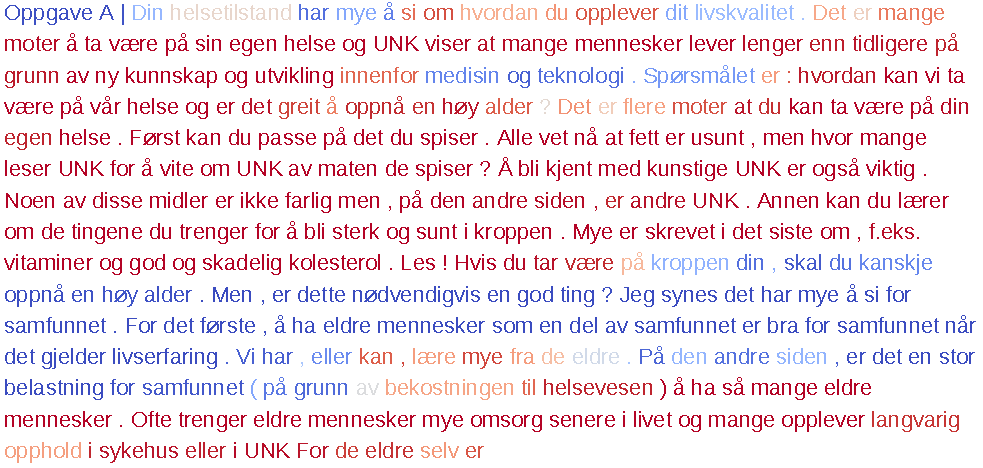
\includegraphics[width=\textwidth]{h0169-eng}
  \caption[Attention in a text by an English speaker]{
    Attention values of NLI classifier on excerpt from ASK text h0189. L1 is
    English, CEFR score B2.
  }
  \label{fig:eng-attention}
\end{figure}

\begin{figure}
  \centering
  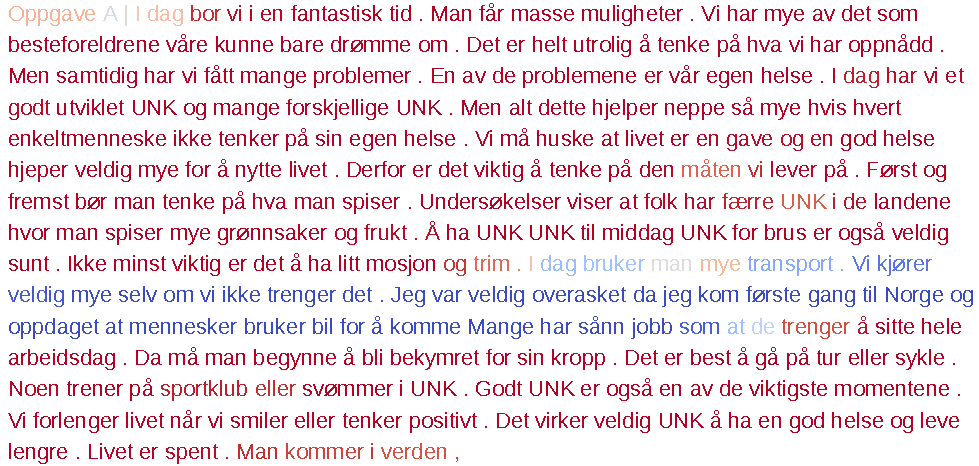
\includegraphics[width=\textwidth]{h0185-rus}
  \caption[Attention in a text by a Russian speaker]{
    Attention values of NLI classifier on excerpt from ASK text h0186. L1 is
    Russian, CEFR score B1/B2.
  }
  \label{fig:rus-attention}
\end{figure}

The Russian speaker's text (fig. \ref{fig:rus-attention}) is almost entirely
high-attention in this excerpt. There is a section of low-attention, around
three sentences long, in the middle of the excerpt. We can therefore not pick
out specific features that the model seems to focus on.

One of the findings in \textcite{pepper2012} was that speakers of Slavic
languages tend to use fewer indefinite articles. In this excerpt we see an
example of the opposite, for instance in the twice occurring `*en god helse'
(\emph{*a good health}). `Helse' (\emph{{health}}) is an uncountable noun,
and should therefore not have an indefinite article, neither in Norwegian nor
English. While this runs counter to the general trend for learners with
Slavic \acp{L1}, it could perhaps be interpreted as a case of
hypercorrection, i.e. a conscious effort to use articles that results in
false positives.

\begin{figure}
  \centering
  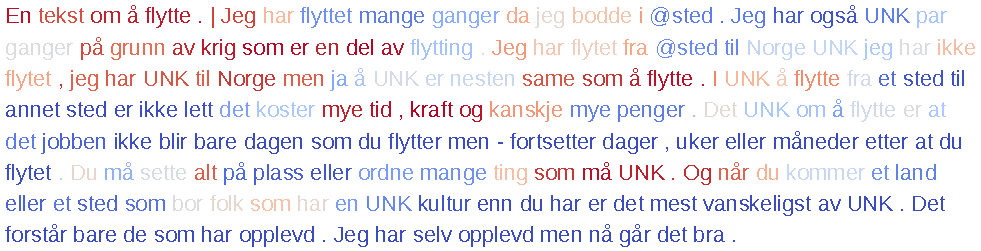
\includegraphics[width=\textwidth]{s0546-som}
  \caption[Attention in a text by a Somali speaker]{
    Attention values of NLI classifier on full ASK text s0621. L1 is Somali,
    CEFR score A2.
  }
  \label{fig:som-attention}
\end{figure}

In the Somali speaker's text (fig. \ref{fig:som-attention}), most of the text
has low attention, except for shorter segments with high attention. However,
the attention is not highest on the most obvious mistakes.

In \textcite{pepper2012}, Somali speakers were found to use the auxiliary
`skal' (\emph{shall/will}) and the pronoun `jeg' (\emph{I}) more frequently
than native Norwegian speakers and several other L1 groups.
\citeauthor{pepper2012} suggested that the frequency of `skal' partly might
be explained by topic bias, since some essay prompts were about the future,
and `skal' is often involved with the future tense. This excerpt is not one of
these texts, and concerns a past experience. Thus, it is not surprising that
it contains no occurrences of `skal'. On the other hand, `jeg' is indeed a
frequent word, occurring five times in the course of a rather short text.

\begin{figure}
  \centering
  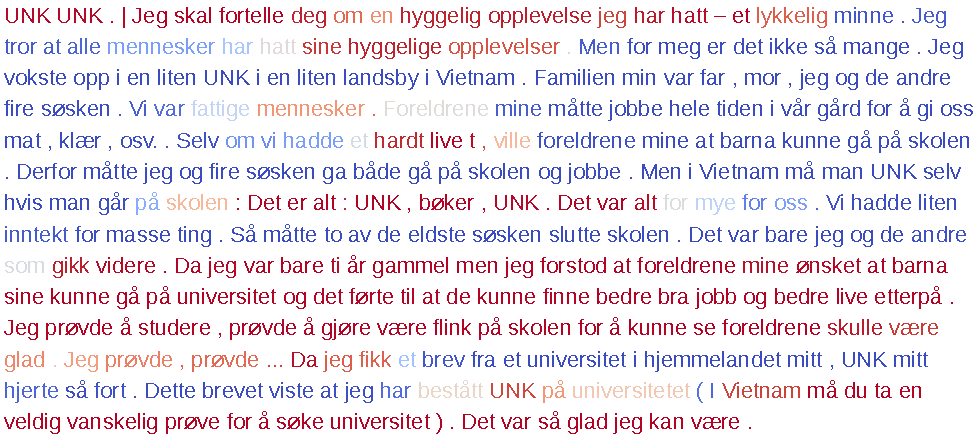
\includegraphics[width=\textwidth]{s0628-vie}
  \caption[Attention in a text by a Vietnamese speaker]{
    Attention values of NLI classifier on excerpt from ASK text s0180. L1 is
    Vietnamese, CEFR score B1/B2
  }
  \label{fig:vie-attention}
\end{figure}

In the Vietnamese speaker's text (fig. \ref{fig:vie-attention}), the word
Vietnam appears three times. This should be a very informative word, as it is
likely that when someone mentions a country in this context, it is their
country of origin. Two of the occurrences have low attention, and one (on the
second-to-last line) has high attention.

Within the high-attention segments, we find a couple of places were the V2
word order in Norwegian shows up. V2 word order is a typological feature of
Norwegian and several other Germanic languages that is challenging to acquire
for many learners.

In one case in this excerpt, `Da jeg var bare ti år` (\emph{Then I was only
ten}), the learner gets the word order wrong (`jeg' and `var' should switch
places), but in another case, `I Vietnam må du ta en [...] prøve' (\emph{In
Vietnam you have to take a test}), they correctly apply V2 word order. Both
these places occur with high attention values, but we cannot say with
certainty that the model actually picks up V2 errors. In this excerpt, there
are also several places with V2 word order that have low attention, for
instance `Så måtte to […] søsken slutte' (\emph{Then two […] siblings had to
quit}). \todo{discussion, attention here}


\subsection{Latent space}

We can use dimensionality reduction methods such as $t$-SNE or \ac{PCA} in
order to see if the intermediate representation of documents prior to the
final classification layer positions documents that should be similar close
to each other. In figure \ref{fig:pca-rnn-cefr} we have taken the documents
in the dev set and computed these representations using a BiGRU, then run
them through the PCA algorithm\footnote{We used the implementation in
Scikit-learn\autocite{scikit-learn}.} in order to project them down to two
dimensions. The resulting dimensions are the two axes that account for most
of the variance in the data. Additionally, the components are uncorrelated
with each other.

\begin{figure}
  \centering
  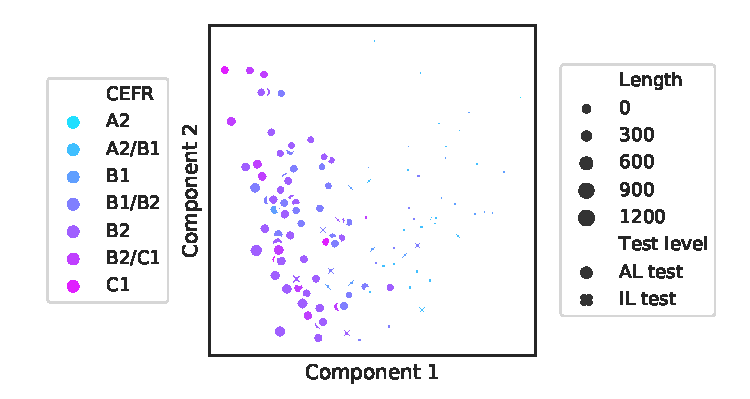
\includegraphics{pca-rnn-cefr}
  \caption[PCA plot of the vector representations of documents]{
    Each document in the dev set is plotted according to its two principal
    components after PCA dimensionality reduction. Marker size and shape
    corresponds to document length and test level, respectively.
  }
  \label{fig:pca-rnn-cefr}
\end{figure}

We see that the first component, which corresponds to the horizontal axis in
the plot, maps closely to the length of the document. The long essays,
indicated by the size of the markers, are on the left hand side of the plot.
These are overwhelmingly from the AL test. The right hand side of the plot is
dominated by texts from the IL test, plotted with crosses, and the size of
the markers indicate that these texts are small. The second component of the
plot, on the other hand, does not seem to be interpretable in terms of CEFR
score, essay length or test level.

As previously discussed, there is a correlation between the length of essays
and the proficiency score, as well as the test level (IL level or AL level).
The system learns to see the length of the essay, likely by the presence of
padding tokens in short essays. Therefore, it learns a feature which is
strongly correlated with the output, namely proficiency labels.


\section{Conclusion}

We implemented CNN and RNN classifiers.
Error analysis and visualization of attention values.
Experiments with pure NLI.
Analyzed the representation of documents in latent space.

Our experiments with \ac{CNN} models confirmed what we saw in the previous
chapter regarding nominal classification versus regression, namely that
regression gives the best results for the \ac{AES} task on this dataset.

Our \ac{RNN} experiments gave results on the task which clearly improved on
our baseline systems.


\section{Ethical considerations}

Language testing is a high-stakes setting. Often, an official language
proficiency certificate is needed in order to be admitted to a study
programme or gain employment, for instance. The high stakes involved means
that the grading of a language test should ideally be transparent and
explainable, something many modern machine learning based models struggle to
achieve.

Even if a computer essay grading system is not used for grading an official
test, it may indirectly influence a language learner's decision to take a
test at a certain time. As established, language testing can be inconvenient
for those taking it, since they have to get to the testing location, pay a
fee, etc.

Language testing is in some places a requirement for gaining citizenship, a
practice that has been criticized [citation needed].

Native language identification also raises ethical concerns. Assumptions
about the dependence of native language and country of origin has been used
as arguments in asylum cases. These assumptions are often wrong, and if
automatic native language identification technologies are easily accessible
they may increase the occurrence of this practice.
This needs better references, but here's 
\href{https://en.wikipedia.org/wiki/Language_analysis_for_the_determination_of_origin}{Wikipedia on LADO}. 


\chapter*{Acronyms}

\begin{acronym}[CBOW]
  \acro{AES}{Automated essay scoring}
  \acro{API}{Application programming interface}
  \acro{CEFR}{Common European Framework of Reference for Languages}
  \acro{CBOW}{Continuous bag of words}
  \acro{CNN}{Convolutional neural network}
  \acro{GRU}{Gated recurrent unit}
  \acro{LADO}{Language analysis for the determination of origin}
  \acro{LDA}{Linear discriminant analysis}
  \acro{LSTM}{Long short-term memory}
  \acro{ML}{Machine learning}
  \acro{MLP}{Multi-layer perceptron}
  \acro{NLI}{Native language identification}
  \acro{NLP}{Natural language processing}
  \acro{POS}{Part of speech}
  \acro{REST}{Representational state transfer}
  \acro{QWK}{Quadratic weighted Kappa}
  \acro{ReLU}{Rectified linear unit}
  \acro{RNN}{Recurrent neural network}
  \acro{SLA}{Second language acquisition}
  \acro{SVM}{Support vector machine}
  \acro{XML}{Extensible markup language}
\end{acronym}
% \chapter*{Abstract}

\backmatter{}

\printbibliography

\end{document}
